%% 
%% Copyright 2007-2020 Elsevier Ltd
%% 
%% This file is part of the 'Elsarticle Bundle'.
%% ---------------------------------------------
%% 
%% It may be distributed under the conditions of the LaTeX Project Public
%% License, either version 1.2 of this license or (at your option) any
%% later version.  The latest version of this license is in
%%    http://www.latex-project.org/lppl.txt
%% and version 1.2 or later is part of all distributions of LaTeX
%% version 1999/12/01 or later.
%% 
%% The list of all files belonging to the 'Elsarticle Bundle' is
%% given in the file `manifest.txt'.
%% 

%% Template article for Elsevier's document class `elsarticle'
%% with numbered style bibliographic references
%% SP 2008/03/01
%%
%% 
%%
%% $Id: elsarticle-template-num.tex 190 2020-11-23 11:12:32Z rishi $
%%
%%
\documentclass[preprint,12pt]{elsarticle}

% \usepackage[UTF8]{ctex}
% \usepackage{xeCJK} % 该命令与上一行等价

%% Use the option review to obtain double line spacing
%%\documentclass[authoryear,preprint,review,12pt]{elsarticle}

%% Use the options 1p,twocolumn; 3p; 3p,twocolumn; 5p; or 5p,twocolumn
%% for a journal layout:
%% \documentclass[final,1p,times]{elsarticle}
%% \documentclass[final,1p,times,twocolumn]{elsarticle}
%% \documentclass[final,3p,times]{elsarticle}
%% \documentclass[final,3p,times,twocolumn]{elsarticle}
%% \documentclass[final,5p,times]{elsarticle}
%% \documentclass[final,5p,times,twocolumn]{elsarticle}

%% For including figures, graphicx.sty has been loaded in
%% elsarticle.cls. If you prefer to use the old commands
%% please give \usepackage{epsfig}

%% The amssymb package provides various useful mathematical symbols
\usepackage{amssymb}
\usepackage{amsmath}
\usepackage{tabularx}
\usepackage{algpseudocode}
\usepackage[margin=3cm]{geometry}
\usepackage{algorithm2e}
\usepackage{textgreek}
\usepackage{color}
\usepackage{booktabs}
\usepackage{geometry}
\usepackage{makecell}
\usepackage{graphicx} 
\usepackage{caption} 
\usepackage{subcaption} 


\geometry{left=1in, right=1in, top=1in, bottom=1in}

%% The amsthm package provides extended theorem environments
%% \usepackage{amsthm}

%% The lineno packages adds line numbers. Start line numbering with
%% \begin{linenumbers}, end it with \end{linenumbers}. Or switch it on
%% for the whole article with \linenumbers.
%% \usepackage{lineno}

\journal{Journal of Manufacturing Systems}

\begin{document}

\begin{frontmatter}

%% Title, authors and addresses

%% use the tnoteref command within \title for footnotes;
%% use the tnotetext command for theassociated footnote;
%% use the fnref command within \author or \address for footnotes;
%% use the fntext command for theassociated footnote;
%% use the corref command within \author for corresponding author footnotes;
%% use the cortext command for theassociated footnote;
%% use the ead command for the email address,
%% and the form \ead[url] for the home page:
%% \title{Title\tnoteref{label1}}
%% \tnotetext[label1]{}
%% \author{Name\corref{cor1}\fnref{label2}}
%% \ead{email address}
%% \ead[url]{home page}
%% \fntext[label2]{}
%% \cortext[cor1]{}
%% \affiliation{organization={},
%%             addressline={},
%%             city={},
%%             postcode={},
%%             state={},
%%             country={}}
%% \fntext[label3]{}

\title{An Edge Intelligence-based Model Deployment Method for CNC Systems}

%% use optional labels to link authors explicitly to addresses:
%% \author[label1,label2]{}
%% \affiliation[label1]{organization={},
%%             addressline={},
%%             city={},
%%             postcode={},
%%             state={},
%%             country={}}
%%
%% \affiliation[label2]{organization={},
%%             addressline={},
%%             city={},
%%             postcode={},
%%             state={},
%%             country={}}


\author[ucas,sict]{Zheng Zhou}
\ead{zhouzheng18@mails.ucas.ac.cn}

\author[ucas,casnc]{Dong Yu\corref{cor1}}
\ead{yudong11@sict.ac.cn}

\author[ucas,sict]{Meng Chen}
\ead{chenmeng@sict.ac.cn}

\author[ucas,sict]{Yusong Qiao}
\ead{qiaoyusong21@mails.ucas.ac.cn}

\author[ucas,casnc]{Yi Hu}
\ead{huyi@sict.ac.cn}

\author[ucas,sict]{Wuwei He}
\ead{hewuwei@sict.ac.cn}

\cortext[cor1]{Corresponding author: Dong Yu}

\affiliation[ucas]{organization={University of Chinese Academy of Sciences},
            addressline={Beijing 100049}, 
            % city={Beijing},
            % postcode={100049}, 
            country={PR China}}

\affiliation[sict]{organization={Shenyang Institute of Computing Technology, Chinese Academy of Sciences},
            addressline={Shenyang 110168}, 
            % city={Shenyang},
            % postcode={110168}, 
            country={PR China}}

\affiliation[casnc]{organization={Shenyang CASNC Technology Co., Ltd.},
            addressline={Shenyang 110168}, 
            % city={Shenyang},
            % postcode={110168}, 
            country={PR China}}



% \author[1]{V. {{\=A}}nand Rawat}
% \ead{rawat@mail.com}

% \author[1,3]{T. Rishi Nair}
% \ead{nair@mail.com}

% \author[2]{Han Theh Thanh \corref{cor1}}
% \ead{thanh@mail.com}

% \address[1]{Indian \TeX{} Users Group, Trivandrum 695014, India}
% \address[2]{Sayahna Foundation, Jagathy, Trivandrum 695014, India}
% \address[3]{\TeX{} Users Group, Providence, MA, USA}

% \cortext[cor1]{Corresponding author}

% \affiliation{organization={},%Department and Organization
%             addressline={}, 
%             city={},
%             postcode={}, 
%             state={},
%             country={}}

\begin{abstract}
%% Text of abstract
\textcolor{black}{Intelligent manufacturing has garnered widespread attention due to its potential to enhance production efficiency and product quality. However, effective resource management remains crucial and challenging, particularly in real-time data processing and task optimization. In response to the shortcomings of existing task offloading solutions regarding network latency and resource limitations, this paper introduces a novel framework for task offloading based on reinforcement learning. This framework dynamically enhances the execution efficiency of neural network tasks and resource allocation within the synchronized control of numerical control systems. Furthermore, this study incorporates digital twin technology further to augment the system's response speed and processing capabilities. Empirical research has demonstrated the significant advantages of the proposed method in reducing computational delay and enhancing processing efficiency. These improvements enhance operational flexibility and ensure efficient system performance in resource-constrained environments. Experimental results indicate that the proposed algorithm surpasses various existing technologies in latency optimization within the experimental benchmark environment.}

\end{abstract}

%%Graphical abstract
%%\begin{graphicalabstract}
%%
\includegraphics[width=\textwidth]{pic/1.pdf}
%%\end{graphicalabstract}

%%Research highlights
% \begin{highlights}
% \item Research highlight 1
% \item Research highlight 2
% \end{highlights}

\begin{keyword}
%% keywords here, in the form: keyword \sep keyword
CNC system \sep Edge intelligence \sep Digital twin \sep Task offloading \sep Cloud-edge collaboration
%% PACS codes here, in the form: \PACS code \sep code

%% MSC codes here, in the form: \MSC code \sep code
%% or \MSC[2008] code \sep code (2000 is the default)

\end{keyword}

\end{frontmatter}

%% \linenumbers

%% main text
\section{Introduction}

%%With the rapid advancement of next-generation information technologies and deep integration with advanced manufacturing techniques, the traditional manufacturing industry is significantly transforming toward intelligent manufacturing \cite{wang2021smart}.  Edge Computing (EC) and Artificial Intelligence (AI) technologies are instrumental in this transformation.  Especially in enhancing intelligence in numerical control systems, the application of these technologies has garnered widespread theoretical attention and achieved notable practical accomplishments.  However, current research applications in numerical control systems primarily focus on data collection and analysis.  There remains a substantial gap in modeling, implementing, and deploying edge intelligence methods\cite{liu2020method,guo2020research}.  This gap hinders the comprehensive development of the intelligent manufacturing sector and represents a critical issue that urgently requires resolution.
\textcolor{black}{With the advent of Industry 4.0, smart manufacturing has become the cornerstone of innovative development in the manufacturing sector\cite{sahoo2022smart}. Against this backdrop, as a critical technology in the manufacturing process, the level of intelligence in numerical control (NC) systems directly influences manufacturing efficiency and product quality\cite{rabiei2023comprehensive}. However, despite existing NC systems possessing specific automation and intelligent capabilities, they still face challenges in achieving efficient real-time monitoring and dynamic task optimization. Particularly under conditions where edge computing resources are limited, and applications demand low latency, effectively managing task offloading and system optimization has become a pressing issue.\cite{zhang2022dependent,avan2023state,chakraborty2022intelligent}}


\textcolor{black}{Current research primarily focuses on harnessing traditional edge computing and artificial intelligence technologies to enhance the performance of numerical control systems. However, these technologies still exhibit limitations in practical applications. For instance, existing task offloading algorithms often fail to fully leverage the benefits of edge intelligence, resulting in ineffective enhancements in computational efficiency and reduced response latency\cite{hortelano2023comprehensive}. Moreover, the prevailing strategies frequently lack the flexibility and adaptability necessary to effectively minimize response times in dynamically changing production environments, particularly in industrial settings characterized by large data volumes and frequent network status fluctuations\cite{acheampong2023review}. Especially under conditions of high workload or network congestion, these systems are often unable to rapidly adjust resource allocation or processing strategies, thus failing to prevent data processing bottlenecks or increased delays. The absence of a systematic approach to effectively integrate edge computing and artificial intelligence to support real-time monitoring and optimization of numerical control systems in an edge intelligence environment further exacerbates these issues\cite{kristiani2024intelligent}. Consequently, researching how to solve the real-time monitoring and intelligent optimization problems of numerical control systems in an edge intelligence setting through innovative model deployment methods and algorithms becomes crucial. This includes developing intelligent algorithms capable of responding in real time to environmental changes and automatically optimizing task offloading decisions, which is vital for enhancing the practical effectiveness and reliability of edge computing, ensuring the system maintains optimal response speed and processing efficiency under various operational conditions.}

The quintessence of this research is the exploration and application of edge intelligence-based deployment methodologies for numerical control system models. By synergizing the essence of digital twins with the pertinent edge intelligence technologies, we have formulated an innovative method for the intelligent modeling of numerical control systems. This method primarily focuses on integrating edge intelligence technologies to facilitate real-time monitoring and intelligent optimization of numerical control systems. In response to the stringent demands for immediacy and accuracy posed by digital twin technology, we have adopted a reinforcement learning-based task offloading algorithm to optimize the performance and responsiveness of numerical control systems.

Through this methodology, our research heralds a new chapter in the era of intelligent manufacturing, mainly providing robust technological support in real-time monitoring and intelligent optimization of numerical control systems.  This advancement propels numerical control systems into a new phase of real-time tracking and intelligent optimization and introduces innovative perspectives to smart manufacturing.  By conducting empirical case studies on intelligent monitoring and learning control optimization in synchronous control scenarios, we have substantiated the practical value of the proposed framework and algorithms in addressing computational and network resource limitations and ensuring the efficiency and accuracy of numerical control systems.  The structure of this document has been meticulously designed to systematically present and discuss the research content, ensuring that readers can thoroughly comprehend our findings and their significant implications in the domain of intelligent manufacturing.

The principal contributions of this article include:

\begin{enumerate}
    \item The study introduces an architecture for numerical control systems tailored for the edge intelligence environment. Leveraging edge intelligence technologies optimizes numerical control systems' performance and efficiency and provides a new methodological framework for constructing and managing digital twin models. Furthermore, the research offers guidance on modeling techniques within related fields.

    \item  In model deployment, it proposes a reinforcement learning-based task offloading algorithm that optimizes the performance and responsiveness of numerical control systems by selecting the optimal computing location for each subtask based on latency and throughput metrics, considering the computational resources and network conditions of edge nodes.

    \item  In model deployment, it proposes a reinforcement learning-based task offloading algorithm that optimizes the performance and responsiveness of numerical control systems by selecting the optimal computing location for each subtask based on latency and throughput metrics, considering the computational resources and network conditions of edge nodes.

    \item The study provides an application case of a digital twin model based on edge intelligence in the intelligent monitoring and learning control optimization of neural networks in synchronous control, validating the practicality and effectiveness of the proposed framework and algorithms.
    
\end{enumerate}

This research unfurls a new chapter for the era of intelligent manufacturing, especially offering substantial technological support in real-time monitoring and intelligent optimization of numerical control systems. The article's structure is meticulously crafted to introduce and discuss the study's content systematically.

The overall structure of the study is divided into six sections, including an introduction. The second section comprehensively reviews related work on model deployment methods for edge intelligence technologies. The third section presents the overall architecture of the CNC system based on edge intelligence. The fourth section describes the optimization theories and methods for the CNC system based on edge intelligence. The fifth section showcases an empirical case study of the CNC system based on edge intelligence. Finally, the sixth section concludes the findings and outlines future research directions.

\section{Related Work}

This section examines critical studies in edge computing, artificial intelligence, and their evolution into edge intelligence. We summarize the developmental trends in these areas and their applications in resource management, task allocation, and intelligent manufacturing.  Special attention is dedicated to the progress of intelligent CNC systems against the backdrop of these technological advancements and the primary challenges they face.  Moreover, this section underscores the necessity and significance of further research, aiming to clarify the contributions and limitations of existing work and provide a solid foundation for our research direction.

\subsection{Edge Computing (EC)}

In edge computing, the effective allocation of resources following the offloading of tasks on terminal devices represents a critical issue. Optimization theory has been pivotal in realizing global optimal solutions for entire chain resource allocation. Bi and colleagues addressed the nonlinear constraint optimization problem with a novel hybrid meta-heuristic algorithm, producing solutions close to the optimum to tackle the challenge of limited resources on intelligent mobile devices\cite{bi2020energy}. Liu and team developed an energy-saving collaborative task computing offloading algorithm based on semi-definite relaxation and random mapping techniques to minimize energy consumption in the Internet of Things (IoT) environment with considerations for task dependency and completion time constraints\cite{liu2019energy}. 
\textcolor{black}{Following explorations in optimization theory that enhanced strategy formulation within edge computing, soft computing methodologies have emerged as innovative approaches for managing uncertainties and augmenting strategic adaptability. In addressing the insufficient balance between exploration and exploitation that multi-objective optimization algorithms face when tackling irregular Pareto frontier problems, Han et al. have introduced a Reinforced Multi-Strategy Multi-Objective Differential Evolution Algorithm (RLMMDE), which significantly improves performance in such scenarios\cite{han2023multi}. In the realm of Constrained Optimization Problems (COPs), Hu et al. have developed a Cooperative Evolutionary Differential Evolution Algorithm augmented by Deep Reinforcement Learning (CEDE-DRL), which enhances efficiency and diversity in complex optimization landscapes through refined operator selection\cite{hu2023deep}. Addressing the carbon-efficient Distributed Blocking Flow Shop Scheduling Problem (CEDBFSP), Zhao and colleagues have implemented the Pareto-based Discrete Jaya Algorithm (PDJaya), which optimizes both total tardiness and carbon emissions, showcasing soft computing as an effective solution in industrial applications\cite{zhao2022pareto}.}
%Concurrently, the Markov Decision Process (MDP) has emerged as the latest trend for solving resource allocation issues. Li and associates proposed a cost-reduction-oriented joint decision-making scheme for task offloading in IoT edge computing, employing an MDP combined with deep Q-learning (MD-DQN) to handle multi-level task offloading and reduce the resource cost associated with task offloading\cite{li2023efficient}. Yang and colleagues explored using MDP to formulate optimal offloading node selection strategies, addressing issues of available bandwidth and mobile device location based on heterogeneous edge servers with the value iteration algorithm (VIA), aiming to select the best offloading node to minimize offloading time in MEC\cite{yang2020offloading}. 
Intelligent methods represented by reinforcement learning have been widely applied in the resource optimization domain to enhance the adaptability of computation offloading and resource allocation in dynamically changing environments. Xiong and the team used an improved deep Q network (DQN) algorithm to alleviate the problem of IoT edge applications in MEC systems sharing and competing for limited virtual resources\cite{xiong2020resource}. Geng and others applied a distributed computing offloading algorithm (DCOM) based on multi-agent deep reinforcement learning to a vehicular-assisted vehicular edge computing network (VAEN), addressing computation-intensive tasks' delay and energy consumption issues\cite{geng2023deep}. Through these diversified applications of edge computing technologies, the methods above effectively resolve problems of resource allocation and task offloading in edge computing, offering efficient and flexible strategies for the resource management of edge intelligent systems.

\subsection{Artificial Intelligence (AI)}

To conserve resources and time while simultaneously amplifying the overall profitability of the production cycle, artificial intelligence technologies have been integrated into CNC machining and monitoring systems, aiming at optimizing CNC operations. In precision multi-axis motion control systems, contour errors present a critical challenge. Huo and colleagues have employed a Nonlinear auto-regressive network with Exogenous inputs (NARX) to predict and compensate for the output position of two-dimensional CNC machine tools\cite{huo2013nonlinear}. However, this method is relatively complex and does not directly forecast contour errors. Hu and the team have effectively enhanced contour performance by implementing a prediction and feedforward compensation strategy proposed by deep GRU neural networks\cite{hu2020deep}. Furthermore, addressing the nonlinear characteristics of tool wear, García-Pérez and others have developed an automated detection system using CNNs in machining aerospace low-pressure turbine casings, significantly improving the accuracy and efficiency of wear assessment\cite{garcia2023cnn}. Ross and colleagues, focusing on the machining of nickel alloys, have tackled the challenge of tool wear detection across varying cutting environments through a transfer learning model\cite{ross2024novel}. In manufacturing quality control, EL Ghadoui and the team have devised an intelligent measurement system that combines deep learning with computer vision, greatly accelerating the speed and accuracy of surface roughness assessments for steel components\cite{el2023intelligent}. Concurrently, Mongan and associates have proposed a methodology based on integrated neural networks, successfully optimizing the CNC milling process, thus enhancing machining efficiency and product quality\cite{mongan2023ensemble}. By harnessing artificial intelligence and deep learning technologies, these studies have effectively addressed challenges in CNC machining optimization, tool wear monitoring, and surface roughness assessment, paving new pathways to elevate production efficiency and product quality.

\subsection{Edge Intelligence (EI)}

To maximize the potential of big data generated at the network edge, Zhou and colleagues introduced the concept of Edge Intelligence (EI), deploying intelligent algorithms near end-users and the network periphery\cite{zhou2019edge}. This approach, grounded in the robust mathematical foundation of edge computing, offers novel perspectives for implementing AI and machine learning algorithms in CNC, particularly enhancing real-time data processing and decision-making capabilities. Nonetheless, the edge-cloud collaborative brilliant machine tool architecture proposed by Lou and others\cite{lou2020intelligent}, while providing fresh insights into real-time data processing and decision-making, still faces challenges in data integration and practical application\cite{liu2020wireless,xu2020edge}. In addressing these challenges, Wu and the team developed FADA, a system based on cloud-fog-edge architecture and ontology, significantly improving data standardization and processing efficiency in intelligent manufacturing\cite{wu2020fada}. Concurrently, Du and colleagues, addressing the issue of high mobility wireless data collection in edge learning, proposed the Fast Analog Transmission (FAT) scheme, which, by supporting spatial multiplexing and direct application in model training, effectively reduces latency and enhances learning accuracy in high mobility scenarios\cite{du2018fast}. Furthermore, Laili and associates, tackling the complexity of cloud-edge-device cooperative task scheduling, introduced a discretized soft actor-critic differential evolution algorithm, reducing overall objectives by up to 30.82\% to 44.35\%, thereby optimizing task scheduling efficiency in distributed production lines and flexible workshops\cite{laili2023dsac}. Additionally, addressing resource management issues in fog computing IoT environments, Wei and the team implemented a joint optimization scheme via nature-inspired actor-critic deep reinforcement learning, effectively reducing average end-to-end latency, improving service response times, and enhancing bandwidth utilization\cite{wei2018joint}. Through these studies, edge intelligence and advanced algorithms elevate data processing efficiency and optimize resource usage, providing new avenues for intelligent manufacturing and real-time decision-making.


The studies above illuminate the advancements made in edge computing, artificial intelligence, and the evolved sector of edge intelligence, offering innovative solutions for resource management, task allocation, and intelligent manufacturing. Despite these achievements, the evolution of intelligent CNC systems continues to face formidable challenges, including the inadequacy of technological expansion from individual applications to system-wide integration, the absence of a unified standard format for multi-source heterogeneous data, optimization issues within decision-making strategies, and the technical challenges associated with the practical integration and application of edge intelligence technologies. These issues highlight the limitations of existing research and delineate the direction for future endeavors, particularly emphasizing the importance of comprehensive monitoring and optimization in intelligent CNC applications. This study aims to address these challenges by proposing an intellectual CNC framework and algorithms, primarily through the application of edge intelligence technologies in smart integration, to propel intelligent numerical control systems into a new era of real-time monitoring and intelligent optimization.

\section{Edge Intelligence-Based CNC System Architecture}
\subsection{Requirements in Intelligent Manufacturing}

The advent of Industry 4.0 heralded a new epoch in intelligent manufacturing, predicated on optimizing the manufacturing process through automation, digitalization, and networking\cite{el2021design}. The intelligence level of numerical control (NC) systems drives this transformation and determines manufacturing efficiency and product quality\cite{yao2019design}. Against the backdrop of intelligent NC systems, edge intelligence technologies have provided new avenues for enhancement and optimization\cite{zhang2022information}. For instance, the trend towards mass customization, facilitated by Information and Communication Technology (ICT), illustrates this shift, with smart factories and intelligent machine tools embodying this concept\cite{kosmowski2022integrated,chen2017smart,lee2020review}, as depicted in Figure 1.

\begin{figure}[hbt]
    \centering
    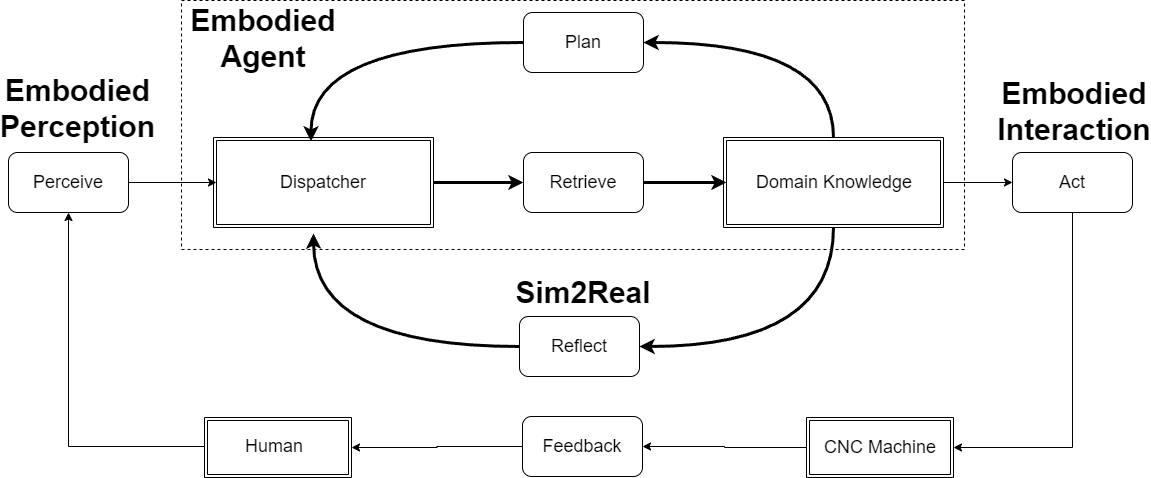
\includegraphics[width=0.8\linewidth]{1.png}
    \caption{Emerging Demands in Intelligent Manufacturing}
    \label{fig: Fig.1}
\end{figure}

As highly integrated electromechanical devices, NC machine tools feature precise control of servo systems and complex trajectory interpolation operations as one of their core technologies\cite{liu2023feedrate}. Servo systems play a crucial role within NC machine tools, using servo motors, amplifiers, and feedback devices to precisely control the machine's motion position, speed, and acceleration, ensuring high accuracy and stability during the machining process. These systems are particularly suited for producing diversified, high-precision, small-batch parts\cite{luo2020hybrid,zhong2020toolpath}. With the development of information and communication technologies, NC machine tools are transitioning from closed to open architectures, gradually increasing their frequency of use in manufacturing workshops\cite{liu2023open,deng2018open}. In the broader context of interconnectedness, the integration of emerging technologies such as the Internet of Things (IoT), artificial intelligence, and edge computing further promotes the intelligence of servo systems, enabling NC machine tools to achieve a more flexible and efficient manufacturing loop, as illustrated in Figure 2. The enhancement of servo systems, coupled with using sensors and edge computing devices, endows NC machine tools with self-perception, self-adjustment, self-prediction, and self-assessment capabilities\cite{ye2020knowledge}. This not only augments the functionality of NC machine tools but also expands their application domains. Furthermore, intelligent NC systems are responding to the following new industrial development demands:

\begin{enumerate}
    \item With the evolution of intelligent manufacturing, NC systems must break down information silos to achieve efficient interconnectivity between devices.

    \item The deluge of data by IoT technologies and the stringent demands for real-time processing pose new challenges to NC systems' immediate data handling and response capabilities.

    \begin{figure}[h]
        \centering
        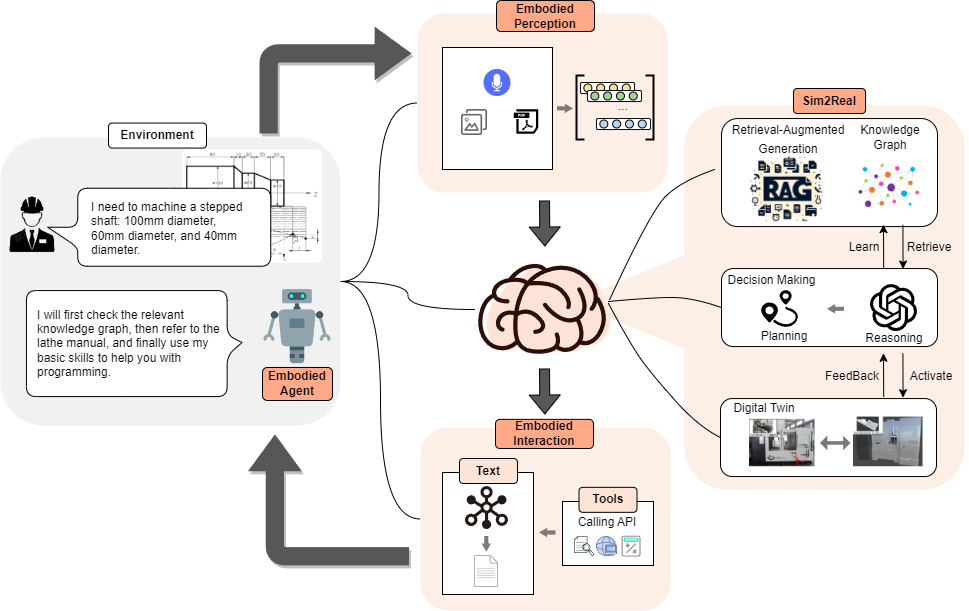
\includegraphics[width=\linewidth]{2.png}
        \caption{Intelligent NC System with Adaptive Control}
        \label{fig: Fig.2}
    \end{figure}

    \item Given the importance of data privacy protection, especially in high-end manufacturing sectors like aerospace, industrial producers are cautious about cloud data processing, preferring local processing and storage of critical information.

    \item The limited resources of industrial sites, along with the pursuit of production accuracy, quality, and efficiency, require servo systems to enhance the production throughput of NC machine tools while ensuring machining precision.
    
\end{enumerate}

\subsection{System Modeling and Structure}
A modular structure plays a pivotal role in the design of numerical control systems. When it comes to the intelligentization of these systems, such an architectural approach enhances their adaptability and scalability and lays a solid foundation for real-time monitoring and operational precision\cite{yu2023edge}.


Within the modular construction of numerical control systems, the synergy between various intelligent elements across modules fosters a dynamic environment for learning and self-optimization, as illustrated in Figure 3. This interplay significantly bolsters the system's adaptability and autonomy. The intelligent elements include:

\begin{itemize}
    \item Perception and Interconnectivity: Sensing the state and environment of the numerical control system through sensors and other data acquisition methods. This information forms the foundation of the intelligent system's decision-making and must be accurately collected and processed.

    \item Digital Twin Models: Virtual replicas of the physical numerical control systems that can simulate and analyze system performance in real-time. Through this mechanism, intelligent systems can anticipate future states or understand the potential impacts of specific actions.

    \item Learning and Modeling: The capability of the intelligent system to learn from its current state and model the situation accordingly. This involves employing deep learning algorithms to identify patterns or anomalous behaviors to assess the system's operational status or maintenance needs.

    \item Optimization and Decision Making: Based on the assessment and diagnosis of the current state, the intelligent system must be able to make decisions and execute actions for optimizing tasks. This could involve adjusting system parameters, initiating maintenance procedures, or altering operational strategies to enhance efficiency and performance.
\end{itemize}

This process manifests in intelligent numerical control systems as continuous data collection by various modules (such as machine status, machining efficiency, and motor positions) to adjust strategies for optimizing system performance. The effectiveness of these improvements is then validated through actual machining outcomes. This cycle ensures that the numerical control systems can self-optimize and adapt to evolving production demands.

\begin{figure}[hbt]
    \centering
    \includegraphics[width=0.85\linewidth]{3.png}
    \caption{Intelligent Elements Modeling Scheme of NC Systems}
    \label{fig: Fig.3}
\end{figure}

In intelligent manufacturing, numerical control systems perform numerous critical functions, such as intelligent monitoring and optimization in synchronous control and trajectory planning for NC machine tools. These functions demand stringent time controls to ensure machining accuracy and efficiency. Under traditional cloud computing models, limitations in network bandwidth and latency could lead to uncertainties in timing delays, affecting the timeliness of real-time data processing and potentially leading to discrepancies between the physical machine tools and their digital twins\cite{liu2023intelligent,xiao2024step}. Adopting edge intelligence methods becomes an essential solution strategy to address this issue, significantly reducing the time required for data transmission and processing by processing data near its source, thereby ensuring data interaction consistency and synchronicity\cite{nain2022towards}. This technology is indispensable for the real-time and accurate execution of numerical control systems. In this context, we have constructed a comprehensive intelligent data processing architecture, as shown in Figure 4. This layered and modular approach enhances the system's flexibility, providing robust technical support for numerical control systems within an intelligent manufacturing environment.

Physical Layer: Primarily consists of NC machine tools and various sensors, acting as the data source, responsible for real-time capture and monitoring of machine operation data. Continuous monitoring of machine states by these sensors collects critical performance parameters. It uploads this raw data directly to the network layer, ensuring comprehensive and timely data collection for precise input to higher-level processing.

Network Layer: Edge nodes and servers within this layer form the vanguard of data processing, undertaking data relay, preliminary processing, and intelligent analysis. Positioned close to the physical sources, edge nodes can preprocess collected data, such as data cleansing and preliminary analysis, to alleviate the load on the cloud. Edge servers further process this data, running advanced algorithms for process optimization, machining simulation, health management, and establishing digital twins, providing essential support for real-time decision-making. This layer's design makes data processing more efficient and responsive, offering immediate and reliable information support for the application layer.

Application Layer: Users access real-time monitoring, fault prediction, and diagnostic services through interactive interfaces connected to the network layer's cloud and edge computing resources. This layer not only presents the analytical outcomes of the network layer but also integrates advanced data processing from the cloud with the immediate decision-making capabilities of edge computing, achieving intelligent control of the production process. Furthermore, through close cooperation with the cloud and edge layers, the application layer can offer rapid feedback and decision support, enhancing the system's autonomy and production efficiency.

\begin{figure}[hbt]
    \centering
    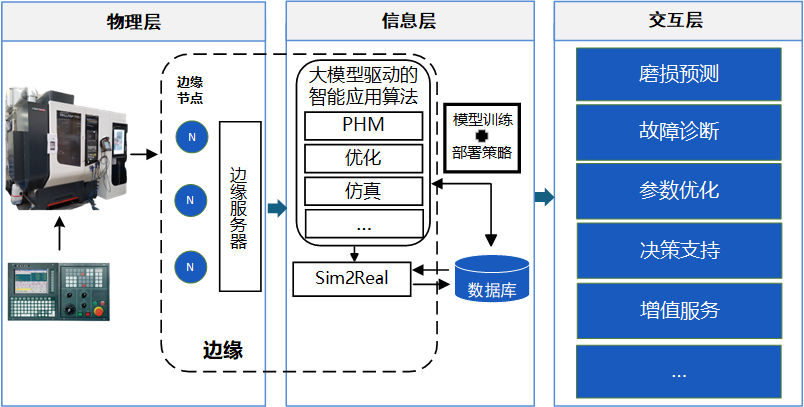
\includegraphics[width=\linewidth]{4.png}
    \caption{Network Topology Diagram}
    \label{fig: Fig.4}
\end{figure}

The real-time perception and processing of data are paramount within the intelligent architecture of numerical control systems.  By deploying various sensors, such as vibration, sound, and temperature sensors, on CNC machine tools, the system facilitates immediate data capture, transmitting it to edge nodes.  Once set with appropriate collection frequencies, these nodes are tasked with data acquisition and preliminary preprocessing.  These nodes communicate with intelligent gateways on edge servers through WebSocket protocols while utilizing GB/T39561\cite{GT3956142020} and OPC UA protocols to handle data from the numerical control systems, ensuring rapid transmission and high data accuracy.  Edge servers, via intelligent gateways, integrate multiple communication protocols, allowing multiple nodes to connect as clients and store information in the GB/T39561 data format compliance using the OPC UA modeling approach, facilitating data subscription and further processing.

In the edge computing architecture, the KubeEdge platform plays a pivotal role, integrating edge servers and nodes under the unified management of the cloud-based Kubernetes cluster. CloudCore in the cloud is responsible for task distribution and scheduling, whereas EdgeCore at the edge ensures local task execution and management\cite{kundroo2022node,kim2023local}. Through containerization, components of neural network models can run efficiently on the most suitable edge computing resources and synchronize with the cloud, maintaining harmony and coordination. This distributed computing structure not only enhances execution efficiency but also guarantees quick responses to real-time data processing. Moreover, customized communication protocols support effective collaboration between edge devices, augmenting the flexibility and response speed of the entire intelligent manufacturing system, thereby bolstering the performance of edge computing.

\subsection{Functional Subcomponents and Model Construction}

\subsubsection{Edge Computing Infrastructure Design}

In the contemporary design of edge computing infrastructure, Figure 5 unveils a modular architecture for the intelligent data processing of numerical control system information, seamlessly integrating the processes of data acquisition, analysis, and application decision-making. Within the perception module, the numerical control system utilizes CNC controllers, sensors, and servo systems to monitor various operational metrics of the machine tools in real-time. Specific attribute data (such as machine status, operational model, and G-code line numbers) are directly connected to the edge server through DLL or industrial communication protocols like MQTT and Modbus; other data (such as vibration signals from the X, Y, and Z axes) require initial transmission to an edge node, where they undergo preprocessing before being relayed to the edge server.

Leveraging the high-performance computing capabilities of the NVIDIA Jetson Xavier NX, the edge server conducts preliminary parsing and structuring of data, facilitating subsequent analysis. The edge server module is designed with modularity in mind to handle various complex analysis tasks adeptly. Guided by information and mechanistic models, this module employs efficient data fusion, analysis, and storage strategies in conjunction with application algorithms, executing advanced algorithms such as tool path optimization to assess the current state of machine tools and predict future maintenance requirements. These analytical outcomes are then instantaneously fed back into production process decisions through the control logic module, ensuring the optimization of operations and maximization of machine tool performance.

The proposed architecture's edge intelligence-based numerical control system model provides critical support for achieving intelligent objectives. This design optimizes dynamic task allocation between edge servers and computing nodes, ensuring the timeliness and efficiency of proximal data processing and effectively alleviating the cloud processing load. By allocating tasks with high immediacy requirements to be executed on edge computing nodes, processing speed is enhanced, and resource allocation is optimized, rendering the design of edge computing infrastructure more efficient and responsive.

\begin{figure}[hbt]
    \centering
    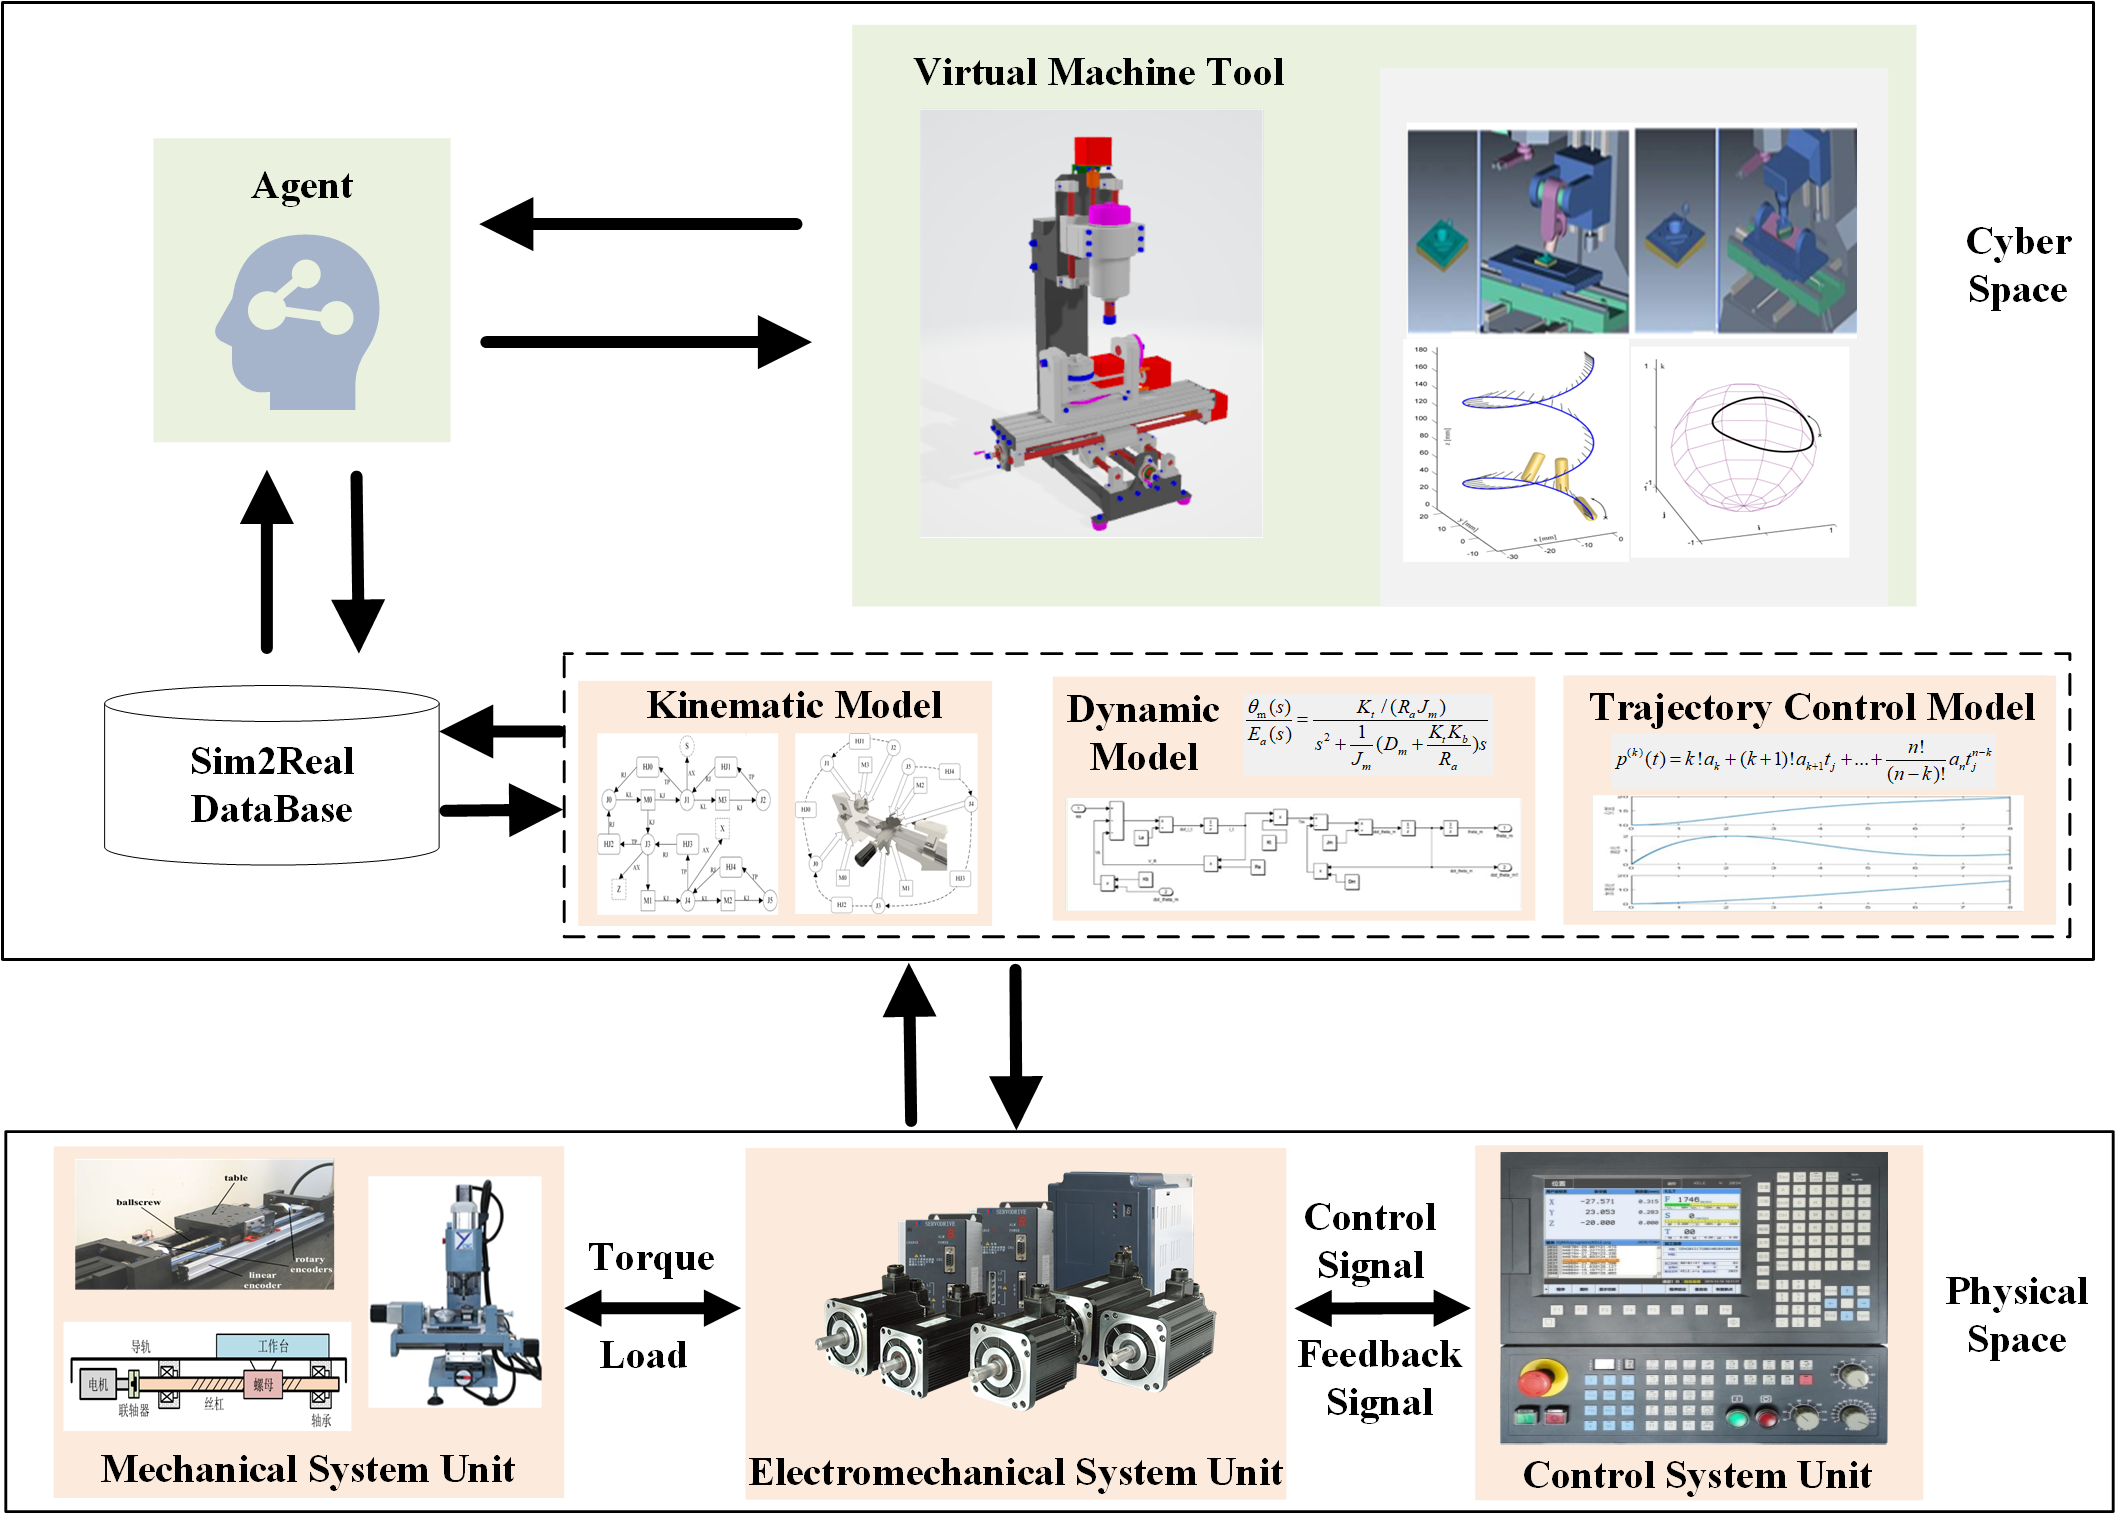
\includegraphics[width=\linewidth]{5.png}
    \caption{Edge Intelligence-Based NC System Structural Model}
    \label{fig: Fig.5}
\end{figure}

\subsubsection{Construction of Information Model (IM) and Mechanistic Model (MM)}

In modern numerical control systems' intelligent and networked architecture, reliance on precise and efficient Information Models (IM) and Mechanism Models (MM) is essential for real-time monitoring and effective management. We can significantly enhance model accuracy and system response efficiency by adopting standardized modeling and simulation techniques, thereby meeting the performance requirements in an edge intelligence environment.

\textbf{Construction of Information Model (IM)}

In constructing the Digital Twin's Information Model (IM) for numerical control systems, the systems themselves and data acquisition devices play a crucial role. Following the GB/T 39561.4-2020 standard, we have conducted a comprehensive analysis of the basic information model of CNC equipment, encompassing static attributes (describing inherent system characteristics), process attributes (reflecting operational characteristics of the system), configuration attributes (necessary configurations for executing tasks), and various components (such as CNC controllers, servo systems, I/O, PLCs, etc.). These elements collectively support the real-time monitoring and efficient management of the numerical control system, as depicted in Figure 6.

\begin{figure}[hbt]
    \centering
    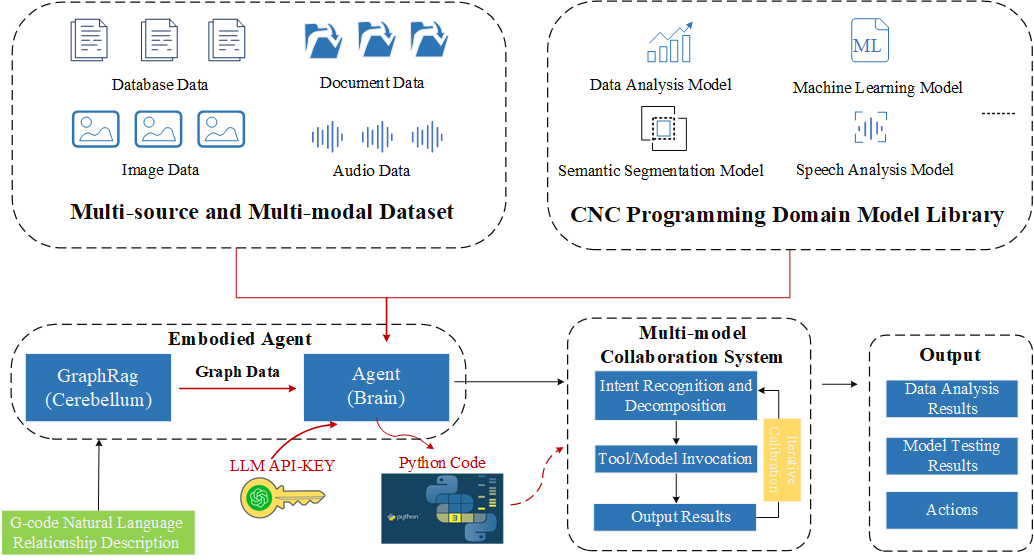
\includegraphics[width=\linewidth]{6.png}
    \caption{Information Model of NC System}
    \label{fig: Fig.6}
\end{figure}

\textbf{Construction of Mechanism Model (MM)}

In precision manufacturing processes, achieving accurate control across multiple axes of CNC machine tools is paramount, directly impacting production precision and efficiency. However, traditional control methods that rely on mechanical adjustments face significant challenges in addressing the non-linearity and dynamic changes during machining processes\cite{youssef2023review,you2021adaptive}. Due to slow response times, these methods often fail to compensate effectively for machining inaccuracies and diminished machine performance. This limitation primarily arises from the traditional control devices' lack of adaptability to real-time changes in machining conditions and mechanical wear; moreover, these control methods are designed for linear systems and do not align with the non-linear dynamical characteristics of CNC machinery. Additionally, there is a noticeable delay in responding to dynamic changes due to slow processing and reaction times. These limitations underscore the constraints of traditional methods in modern precision manufacturing and highlight the necessity of adopting more advanced control strategies to overcome these challenges.

These limitations accentuate the demand for more advanced, intelligent methods. The choice of neural network-based control and monitoring is primarily due to neural networks' ability to handle complex non-linear issues in CNC system operations, especially in scenarios of synchronous control. Unlike traditional control methods, neural networks can learn and identify complex patterns and relationships from data, providing more accurate and dynamic control strategies. This method not only adapts to subtle changes in system behavior but also processes and responds in real-time, ensuring the high precision and efficiency of CNC systems. Furthermore, the real-time monitoring capabilities supported by neural networks continuously optimize operational parameters, reduce manual intervention, and enhance automation levels. Thus, neural network-based monitoring and optimization are ideal for addressing synchronous control issues.

\begin{figure}[hbt]
    \centering
    \includegraphics[width=0.75 \linewidth]{7.png}
    \caption{Edge Intelligence-Based Synchronous Control Monitoring and Optimization Process}
    \label{fig: Fig.7}
\end{figure}

To address the challenges of synchronous control in high-speed, high-precision machining encountered by CNC systems and to overcome the limitations of traditional control methods in handling non-linear dynamic systems, this study employs an advanced model based on deep neural networks. Leveraging their exceptional non-linear modeling capabilities and adaptive learning features, the model can effectively learn optimal strategies for synchronous control from complex currents, speeds, and positional data, as shown in Figure 7. In this process, the neural network plays a crucial role, accurately predicting the CNC system's dynamic error adjustment needs in real-time and automatically optimizing control parameters based on these predictions, thereby achieving high-precision dynamic error compensation. Deploying this deep neural network model on edge computing devices enables real-time monitoring and optimization of CNC systems, significantly enhancing machining efficiency and product quality. The model's feedback learning mechanism also ensures the system can continuously adapt to new working conditions and wear states, maintaining long-term high-performance operation. This approach strengthens the response capability to dynamic changes and enhances the system's adaptability and flexibility, showcasing the immense potential of deep learning-based control strategies in modern precision manufacturing.

To ensure high-precision synchronous control of CNC systems in complex machining environments, this study introduces a set of anomaly detection and adjustment strategies based on deep neural networks. Initially, the calculation formula for anomaly detection thresholds can be expressed as:

\begin{equation}
    G=|P_{actual}-P_{expected}|
    \label{equation:1}
\end{equation}

Equation \ref{equation:1} quantifies the deviation between the actual and expected positions, where D represents the dynamic error between these two points. When this error exceeds a predetermined threshold θ, it is identified as an anomalous state requiring control adjustment. The threshold θ is based on analyzing historical data and understanding mechanical performance, aiming to find a balance between the system's response sensitivity and operational practicality.

Furthermore, to execute the necessary adjustments with precision, this study utilizes an adjustment calculation formula as follows:

\begin{equation}
    A=S \times G
\end{equation}

The adjustment amount A, calculated through Equation 2, directly correlates with the actual adjustment actions the system needs to undertake to ensure optimal outcomes. Here, S acts as a sensitivity factor, adjusting the proportion of the adjustment amount based on the magnitude of dynamic error D, allowing the system to respond flexibly under actual operational conditions. This strategy enhances the NC system's ability to handle nonlinear issues. It improves adaptability and precision when facing complex machining tasks, ensuring high consistency between machining efficiency and product quality.

\subsection{Edge Intelligence-Based Model Deployment Method}

In the realm of numerical control systems, the deployment of models based on edge intelligence is achieved through a series of meticulously orchestrated steps. As illustrated in Figure 8, initially, upon sensing data from the numerical control system, edge nodes identify available computing resources through service discovery, laying the groundwork for subsequent operations. In the neural network task segmentation phase, complex deep learning models are divided into multiple neural network subtasks, maintaining the functional integrity of each segment to facilitate effective execution across various computing environments. Intelligent offloading decisions are made based on task latency and throughput metrics, automatically selecting whether to offload to high-performance devices and which subtasks to offload. The task transmission phase involves securely and efficiently transferring selected tasks to the designated computing devices. These devices then undertake the responsibility of computation execution, processing the tasks allocated to them. Ultimately, the processed results are relayed back to the edge nodes to be fed back into the production process or for further analysis, thereby completing a cycle of model deployment based on edge intelligence.

\begin{figure}[hbt]
    \centering
    \includegraphics[width=0.32\linewidth]{8.png}
    \caption{Fundamental Process of Computational Offloading in NC Systems}
    \label{fig: Fig.8}
\end{figure}

Within our edge intelligence-based numerical control system application model deployment environment, we define a computation offloading problem to optimize task processing latency and resource utilization. They are considering a set \(N\), where \(N=\{N_i |i=1,2,...,n\}, N_i\) represents an independent neural network subtask and a total of n subtasks; these subtasks must be processed on the intelligent numerical control system's edge nodes or edge servers. Each subtask requires a decision on whether its computation must be offloaded to the edge server. To align decision outcomes closer to achieving an optimal task offloading partitioning that balances latency, throughput, and latency threshold, a mathematical model is introduced into the environment as part of the reward, aiming to maximize subtask real-time strategy performance and optimal allocation of computing resources under the oversight of the observer. Offloading decisions must consider the dependencies between tasks, the dynamic nature of network conditions, and each neural network layer's computational and data transmission requirements, simultaneously flexibly improving the original approach that solely relied on a one-size-fits-all mathematical model.

\subsubsection{Resource Allocation Optimisation Modeling}

In edge intelligence-based numerical control systems, modeling for optimizing network and computing resource allocation is a critical component in reducing service latency and ensuring service quality. In our offloading environment, we model different resource allocation optimization models involving network and computation.

\textbf{Network Resource Allocation Optimisation Model}

Under the "cloud-edge-device" architecture, each edge node can process each subtask locally or offload the computational task to the edge server through the channel. The computation offloading strategy for subtasks within edge nodes can be defined as follows:

% \begin{equation}
%     a_i\left\{
%         \begin{aligned}
%             &0,&Local \ Computing\\
%             &1,&Local \ Offloading
%         \end{aligned}
%     \right.
% \end{equation}

\begin{equation}
a_i = \left\{
    \begin{aligned}
        &0, && \text{Local Computing} \\
        &1, && \text{Local Offloading}
    \end{aligned}
\right.
\end{equation}

Thus, \(a_n=(a_1,a_2...,a_n)\) represents the set of all subtask computation offloading strategies for the edge node.

Based on the Shannon capacity formula, the uplink transmission rate during the offloading of computational tasks from edge nodes to edge servers is

\begin{equation}
    C_{i,up}(a_i)=Klog_2(1+S_{i,up}/N_i)
\end{equation}

Similarly, the downlink transmission rate is

\begin{equation}
    C_{i,down}(a_i)=Klog_2(1+S_{i,down}/N_i)
\end{equation}

Within this context, \(K\) represents the bandwidth between the edge node and the server. For \(S_{i, up}=q_{i, up}g_{i, up}\) and \( S_{i, down}=q_{i, down} g_{i, down}, q_{i\\, up}\) and \(q_{i, down}\)  denote the transmission power of the edge node and edge server, respectively, while \(g_{i, up}\) and \(g_{i, down}\) correspond to the uplink and downlink channel gains. \(N_i=\sigma+\sum_{i\in{N}:a_i=a_n}q_i g_i\), where  \(\sigma\) represents the background white noise interference, and  \(\sum_{i\in{N}:a_i=a_n}q_i g_i\) signifies the communication interference from other channels. The uplink and downlink rates are defined as the maximum throughput in the network transmission task, allowing the channel capacity derived from the Shannon formula to be considered as the maximum possible throughput for this network transmission task.

\textbf{Computational Resource Allocation Optimization Model}

The computational resource allocation optimization model has two modes: edge node computation and edge server computation. The computation-intensive tasks at the edge node can be defined as \(I_i \triangleq B_i\), where \(B_i\) represents the volume of data required by the edge node to complete the computation task.

\begin{itemize}
    \item {\fontsize{11}{\baselineskip}\selectfont \textbf{Edge Node Local Computation}}
\end{itemize}

When the computation results from the edge server need to be transmitted back to the edge node, the edge server transmits the results to the edge node through the channel, defining the time cost of the download transmission process as:

\begin{equation}
    t_{i,down}^{edge} (a_n )=\frac{B_i}{C_{i,down} (a_n )} 
\end{equation}


When the decision is for the edge node to compute locally, subtask i is executed on the edge node to perform computation task \(I_i\). Let \(f_i^edge\) represent the computational capability of the edge node (i.e., the CPU clock frequency in Hz). Thus, the execution time for performing computation task \(I_i\) on the edge node is:

\begin{equation}
    t_{i,exe}^{edge}=\frac{B_i}{f_i^{edge}}
\end{equation}

The total cost of computation at the edge node is:

\begin{equation}
    K_n^{edge} {a_n}=\lambda_n^t (t_{n,down}^{edge} (a_n )+t_{n,exe}^{edge} )
\end{equation}


Here, \(\lambda^t_n \in (0,1)\) denotes the computational time weight assigned by edge node n at the decision-making time. It sets the value based on the sensitivity requirement to latency in its scenario, thereby dynamically adjusting the system's overall cost.

\begin{itemize}
    \item {\fontsize{11}{\baselineskip}\selectfont\textbf{Edge Server Computation}}
\end{itemize}

When the edge node decides to compute at the edge server, the edge node offloads the computation-intensive task to the edge server through the channel, defining the time cost of the offloading transmission process as:

\begin{equation}
    t_{i,up}^{server} (a_n )=\frac{B_i}{C_{i,up} (a_n )} 
\end{equation}

The computational capability of the edge server, represented by the clock frequency \(f_n^c\), then the time to execute computation task \(I_n\) is:

\begin{equation}
    t_{i,exe}^{server}=\frac{B_i}{f_i^{server}}
\end{equation}

The total cost of computation at the edge server is:

\begin{equation}
    K_n^{server} {a_n}=\lambda_n^t (t_{n,up}^{edge} (a_n )+t_{n,exe}^{server} )
\end{equation}

Here, \(\lambda_n^t\in(0,1)\). Since many offloaded computation-intensive tasks involve a large volume of computational input data. In contrast, the computational feedback results are often minimal, and the time cost of feedbacking the computation results to the edge node can be disregarded.

\subsection{Evaluation Method Based on Integer Linear Programming (MILP)}

Task partitioning is the pivotal step in the evaluation. It aims to identify the optimal division point that balances latency and throughput, allocating tasks before the partition point to the edge node and tasks after it to the edge server\cite{wang2023task}. We employ Mixed Integer Linear Programming (MILP) to address this challenge.

Specifically, the steps for task partitioning are as follows:

\begin{enumerate}
    \item Create a MILP problem with an objective function that aims to minimize the total delay variance, thus combining the effects of delay and throughput. This can be expressed in the following equation:

    \begin{equation}
    \label{eq. 12}
        latency_{diff}=\sum^n_{t=1}|(t_{i,exe}^{edge}-t_{i,exe}^{server})\cdot y_i|
    \end{equation}

    Here, \(n\) denotes the number of tasks, \(t_{i,exe}^{edge}\) and \(t_{i,exe}^{server}\), respectively, signify the execution times of task \(i\) on the edge node and edge server, and \(y_i\) is a binary decision variable indicating whether task \(i\) is partitioned after that.

    \item Introduce constraints to ensure the total latency does not exceed an acceptable threshold. These constraints consider the latency of each task on edge devices and cloud servers and data transmission latency. The specific constraints are as follows:

    \begin{equation}
    \label{eq. 13}
    latency_i^{edge}=\sum^i_{j=1}t_{j,exe}^{edge}+t_{i,up}^{server}(a_n)
    \end{equation}

    \begin{equation}
    \label{eq. 14}
        latency_i^{server} = \sum^n_{j=j+1}t_{j,exe}^{server}+N\cdot t_{i,down}^{edge}(a_n)
    \end{equation}
    
    \begin{equation}
    \label{eq. 15}
        latency_i^{edge}\cdot y_i+latency_i^{server}\cdot(1-y_i)\leq latency_{tolerable}
     \end{equation}

    Here, \(latency_i^{edge}\) and \(latency_i^{server}\) represent the latency of task \(i\) on the edge device and edge server, respectively, \(t_{i,up}^{server}(a_n)\) and \(t_{i,down}^{edge}(a_n)\) denote the data uplink and downlink transmission latency of task \(i\), and \(latency_{tolerable}\) is the acceptable total latency threshold.
    
\end{enumerate}

Ultimately, by solving the MILP problem, we obtain the optimal task partition point regarding latency and throughput, along with other crucial information related to the partition, such as total latency, latency on the edge nodes and edge servers, data transmission latency, throughput, etc., thereby deducing the optimal partition point based on latency and throughput.

\section{Design and Application of Intelligent CNC System Offloading Algorithm Based on Reinforcement Learning }

Within the framework of numerical control systems based on edge intelligence, the design and application of Artificial Intelligence (AI) algorithms, particularly methods of Reinforcement Learning (RL), play an essential role. Reinforcement Learning, characteristic of self-exploration and learning, offers unique advantages in addressing the dynamic and uncertain issues within numerical control systems. This section delves into the design and application of algorithms based on reinforcement learning, detailing their implementation in task offloading strategies and system performance optimization.

\subsection{Task Offloading}

Task offloading, a central issue in edge computing scenarios, involves transferring computationally intensive tasks from resource-constrained edge nodes to more resource-abundant servers to enhance computational efficiency and reduce latency. A practical task offloading strategy is crucial for achieving real-time monitoring and optimization in numerical control systems powered by edge intelligence.

\textcolor{black}{The invocation of task offloading algorithms based on reinforcement learning is predicated on meticulous observation and analysis of performance metrics within numerical control systems. When these systems encounter resource allocation challenges, such as intensified competition for computational resources or rapidly changing task processing requirements, this paper contemplates optimizing decision-making through reinforcement learning. Several key indicators are established as triggers for invoking reinforcement learning. The most intuitive among these is the ratio of task waiting time to system processing capacity; when this ratio exceeds a predetermined threshold, such as 20\% above the system's average processing capability, it indicates significant processing pressure. Under such circumstances, reinforcement learning optimizes the task offloading strategy, alleviating delays and enhancing resource utilization efficiency.Moreover, the disparity between data transmission and processing rates is a crucial consideration; a notable increase in the proportion of data transmission delays to overall task processing time, reaching or exceeding 30\%, suggests that network conditions may substantially impact task execution efficiency. At this point, the reinforcement learning algorithm is invoked to reevaluate and optimize the scheduling strategy between data flows and computational tasks. By quantifying these indicators, this paper accurately identifies when to leverage the capabilities of reinforcement learning to achieve a more efficient and flexible operational strategy for numerical control systems.}

\textcolor{black}{Throughout the entire process of employing reinforcement learning to optimize task offloading in numerical control systems, persistent monitoring of system states marks the inception. This monitoring includes the real-time collection of vital performance indicators such as computational load and network bandwidth utilization. Upon reaching the predetermined triggering conditions, the system automatically proceeds to the data collection phase, compiling data relevant to the current task—such as task type, resource, and computational demands—to furnish the necessary information for decision assessment. Based on this data, the reinforcement learning model evaluates the current task offloading strategy by computing anticipated reward values to gauge the strategy's effectiveness. The results of this evaluation steer the model's learning process and the revision of decision-making policies, including adjusting policy parameters to maximize long-term rewards. This revised strategy is implemented in practical task offloading decisions to minimize delays, enhance processing speed, and boost resource utilization. This ensures that the numerical control systems can autonomously adjust their strategies to adapt to evolving operational conditions and maintain optimal performance.}

\textcolor{black}{The training of the reinforcement learning model utilized historical operational data from neural networks, harnessing extensive accumulated data on computational task outcomes, network conditions, and task processing times from past sub-tasks. This method trains the model to identify and learn the most effective task offloading strategies. The model can predict the optimal task offloading decisions under varying system states through this approach, thereby minimizing execution delays and enhancing system efficiency. Upon completion of training, the model is integrated into the edge computing layer of the numerical control systems, enabling it to monitor system states in real-time and dynamically adjust task offloading strategies based on current environmental and system performance. This integration not only boosts the system's adaptive capabilities, allowing it to maintain efficient operations amidst constantly changing workloads and network conditions but also ensures that the system continuously learns from each task execution, thereby perpetually refining its decision-making process. This ensures that while maintaining high performance, the intelligent numerical control systems also maximize the utilization of available resources.}

The task initiation phase involves evaluating the computational performance of edge nodes and servers and reviewing designated subtasks. For a data processing task composed of \(n\) subtasks, the system calculates the execution latency of each subtask \(i\) on the edge nodes (\(latency_i^{edge}\)) and the edge servers (\(latency_i^{server}\)) based on theoretical formulas from section 3.4. Since subtasks' processing delay primarily depends on the hardware's computational performance, a one-time latency initialization is sufficient for similar hardware devices. The execution delay of each subtask \(i\) can be determined based on the actual operating performance of the hardware.

The collaborative computing offloading framework based on reinforcement learning proposed in this section aims to dynamically optimize task offloading strategies to adapt to the real-time operational status and changing network environments of numerical control systems. In this framework, an agent is responsible for processing neural network layers and, based on observations such as environmental bandwidth, inference latency of edge nodes and servers, and the actions of previous subtasks, determines the optimal model partitioning decision and pruning weight distribution through a reward function. As illustrated in Figure 9, the system, guided by the agent's decisions, divides the original neural network model into several subtasks. Since solely relying on reinforcement learning for offloading decisions of each subtask might lead to frequent data transmission between closely related tasks, thus increasing the acceptable total latency threshold, the Actor-Critic mechanism is used to assess the decisions, seeking the optimal division method to distribute tasks between edge nodes and servers effectively. This ensures the overall runtime latency remains within acceptable limits, optimizes latency and throughput, and improves the traditional "one-size-fits-all" task partitioning approach. Determining the optimal partitioning strategy is a complex process that depends on the structure of the neural network, the computational capacity of hardware devices, network conditions, and mathematical methods tuned to maximize total rewards. This framework demonstrates how continuous learning and strategy adjustments can optimize response times and computational efficiency in changing operational environments.

\begin{figure}[hbt]
    \centering
    \includegraphics[width=\linewidth]{9.png}
    \caption{Collaborative Computing Offloading Method Based on Reinforcement Learning}
    \label{fig: Fig.9}
\end{figure}

\subsection{Intelligent Agent Interaction Environment Design}

Designing a reinforcement learning algorithm framework suitable for task offloading in numerical control systems is foundational for achieving real-time monitoring and optimization. This section focuses on constructing a reinforcement learning algorithm framework suitable for task offloading in numerical control systems, detailing the agent's interactive environment, including precisely defined state space, action space, reward function, and state transition dynamics.

In the environmental state, the \textbf{State Space} is defined as a multi-dimensional feature set reflecting the current subtask. For the \(i\)th subtask, the state \(s_i\) is represented as:

\begin{equation}
    s_i=[c_i,d_i,i_i,q_i,a_{i-1},a_{i-2} ]
\end{equation}

Here, \(c_i\) represents the computational demand of the current subtask \(i,d_i\) describes the data transmission requirement, \(i_i\) is the current task's index in the queue, \(q_i\) is the number of remaining tasks in the queue, and \(a_{i-1}\) and \(a_{i-2}\) is the action selections of the two preceding tasks. This comprehensive state representation gives the agent a complete environmental view, enabling more informed decision-making.

The \textbf{action space} is set as two discrete options:

% \begin{equation}
%     \label{eq:17}
%     \left\{
%         \begin{aligned}
%             &a_i=0, &Executing\ the \ i^{th}\ subtask \ on \ the\ edge\ node\\
%             &a_i=1, &Executing\ the \ i^{th}\ subtask \ on \ the\ edge\ server
%         \end{aligned}
%     \right.
% \end{equation}

\begin{equation}
    \label{eq:17}
    \left\{
        \begin{aligned}
            &a_i=0, && \text{Executing the } i\textsuperscript{th} \text{ subtask on the edge node}\\
            &a_i=1, && \text{Executing the } i\textsuperscript{th} \text{ subtask on the edge server}
        \end{aligned}
    \right.
\end{equation}



This binary choice of action space is designed to simulate a simplified scenario of task offloading decisions in the real world.

We designed a composite \textbf{reward function} \(R(s_i,a_i)\) incorporating several vital factors to guide the agent toward learning the optimal task offloading strategy. This function considers the latency of task execution (unified here as \(L_i\) for both \(latency_i^{edge}\) and \(latency_i^{server}\))  and throughput (unified here as \(C_i\) for both \(C_{i, up} (a_i)\) and \(C_{i, down} (a_i)\)), along with the cost of action and the Critic's evaluation.

\begin{itemize}

    \item {\fontsize{11}{\baselineskip}\selectfont \textbf{Latency and Throughput Trade-off}}: Initially, latency and throughput are calculated based on the location of task execution (either at the edge node or edge server). The reward function incorporates a trade-off between minimizing latency and maximizing throughput. After normalization, the reward is calculated using the following equation:

        \begin{equation}
            R_i=\alpha log(L_i+1\times 10^{-3})+(1-\alpha)log(C_i+1\times 10^{-3})
        \end{equation}

    \textcolor{black}{In this experiment, \(\alpha\) is a balancing parameter, modulating the significance of delay and throughput within the reward mechanism. The adoption of a logarithmic function (log) is primarily influenced by its nonlinear response characteristics. This method is exquisitely sensitive to minor variations in delay and throughput yet reacts more temperately to substantial changes, enhancing the model's responsiveness to slight performance shifts while ensuring stability in the face of extreme values, thereby facilitating meticulous strategy refinement and optimization. The logarithmic function gracefully smooths out extremities through its natural curve shape, circumventing the significant reward value fluctuations that might otherwise result from using the reciprocals of delay or throughput, thereby ensuring the stability of the reward function and the reliability of computations. Furthermore, this functional form provides positive reinforcement when the delay decreases and throughput increases, aligning perfectly with the optimization goals of minimizing delay and maximizing throughput. To maintain mathematical stability, the experiment incorporates a small constant (1e-3) to prevent the function's input from reaching zero, thus ensuring consistent behavior and operational safety across its entire domain.}

    \item {\fontsize{11}{\baselineskip}\selectfont \textbf{Critic evaluation}}: To increase the diversity of the agent's strategies and introduce external knowledge, our reward function also includes a section based on Critic evaluation. Critic evaluation adjusts the reward based on the degree of alignment between the agent's actions and predefined recommendations.
    

\end{itemize}

The \textbf{State Transition Dynamics (STD)}  are determined based on the current state, actions taken, latency, and throughput. The specific formula is as follows:

\begin{equation}
        s_{i+1}=f(s_i,a_i,L_i,C_i,I_{i+1},q_{i+1})
    \end{equation}

Here, \(f\) represents the state transition function, combining the current state \(s_i\), action \(a_i\), and the latency \(L_i\) and throughput \(C_i\) induced by the action, and updates the task index \(indexI_(i+1)\) and queue length \(q_{i+1}\).

\subsection{Evaluation Algorithm Design}

The task offloading algorithm presented in this paper is designed to efficiently allocate tasks between edge devices and servers to minimize total latency while maximizing throughput. The crux of the algorithm encompasses task partitioning and partition recommendations, coupled with the introduction of Critic evaluation to further refine the agent's decision-making process.

\textbf{Partition Recommendations}

Partition recommendations form a segment of the algorithm aimed at advising the optimal execution location for each task—whether on the edge node or edge server. Utilizing the optimal partition point obtained in the task partitioning step, a suggestion for each task is provided, as depicted in Equation \ref{eq:17}. This results in constructing a binary list, where each element indicates the recommended execution location for the corresponding task. For instance, if the \(i\)th element of the recommendation list is '0', task i should be executed on an edge device; if it is '1', task i should be carried out on a cloud server.



\RestyleAlgo{ruled}
\SetKwComment{Comment}{/* }{ */}

\begin{algorithm}[H]
    \caption{Reward Calculation Algorithm}
    \label{alg:two}
    \KwIn{\\
        $t_{n,up}^{server}(a_n),t_{n,down}^{edge}(a_n)$:Latency data for edge and server\\
        $t_{n,exe}^{server},t_{n,exe}^{edge}$:Data transmission delay data\\
        }
    \textbf{Initialize}\\
            $i$: Current task index\\
            $n$: Total number of tasks\\
            $\alpha$: Weighting factor for latency and throughput in the reward calculation\\
            $\beta$: The extent of the critic's intervention\\
            $L_i$: Latency at the $i^{th}$ task division point \\
            $L_i^{min},L_i^{max}$: Minimum and maximum latencies\\
            $C_i$: Throughput at the $i^{th}$ task division point\\
            $action$: Action taken by the agent (0 for edge, 1 for server)\\
    \textbf{Output}\\$reward$: Calculated reward for the current action\\
        
    \Begin{   
        \eIf{$action==0$}
        {
            $latency\gets$ Calculate the reward of latency consumption according to equation (7)
        }{
            $latency\gets$ Calculate the reward of latency consumption according to equation (10)
        }
        $throughput \gets max(equation(12),(equation(13),N=1))$\\
        $L_i^{min} \gets min(t_{n,exe}^{edge}(a_n)+t_{n,exe}^{edge})$\\
        $L_i^{max} \gets min(t_{n,up}^{server}(a_n)+t_{n,exe}^{server})$\\
        $L^i_{normalized}\gets (L_i-L_i^{min})/(L_i^{max}-L_i^{min})$\\
        $C^i_{normalized}\gets (C_i-L_i^{min})/(L_i^{max}-L_i^{min})$\\
        $reward_{normalized\_actor}\gets -\alpha * log(L^i_{normalized}+1e-3)+(1-\alpha) * log(C^i_{normalized}+1e-3)$
        \If{Critic Evalution enabled}{
        critic\_recommendations$\gets$get\_critic\_recommendations()\\
        matched\_decisions$\gets$ count\_matches(actions\_taken,critic\_recommendations)\\
        $reward_{decisions}\gets $matched\_decisions\\
        $reward_{normalized\_critic}\gets reward_{critic}/n$
        }
        $reward_{total}\gets reward_{normalized\_actor}+\beta * reward_{normalized\_critic}$\\
        Return $reward_{total}$
    }
\end{algorithm}

\clearpage

\textbf{Critic Evaluation}

Critic evaluation is introduced to refine the agent's decision-making further. The Critic assesses the agent's decisions based on the task partition recommendations and allocates rewards based on the number of decisions that match. It calculates the number of tasks that align with the recommendations, assigning rewards to the agent based on the quantity of matched tasks. The greater the number of matches, the higher the reward, encouraging the agent to make decisions following the recommendations. Critic evaluation aids the agent in better adhering to these suggestions, thus further optimizing task partitioning and execution toward achieving the goals of minimizing total latency and maximizing throughput.

\begin{algorithm}[H]
\caption{Critic Evaluation via Partition Function}
\textbf{Input:}\\
    $n$: Total number of tasks\\
    $t_{n,up}^{server}(a_n)$, $t_{n,down}^{edge}(a_n)$: Latency data for edge and server\\
    $t_{n,exe}^{server}$, $t_{n,exe}^{edge}$: Data transmission delay data\\
    P: Predefined tolerable maximum latency\\
\textbf{Output:}\\
    best throughput point\\
\Begin{   
    set $latency_{tolerable}$ to P\\
    initialize model: model $\gets$ LpProblem("optimal-cut", LpMinimize)\\
    \For{$i \leftarrow 1$ \KwTo $N$}{
        $y[i] \gets$ LpVariable("y"+str(i), cat="Binary")\\
    }
    minimize: Objective Function(11)\\
    \For{each task i}{
        $latency_i^{edge} \gets$ calculate latency for edge execution according to formula(12)\\
        $latency_i^{server} \gets$ calculate latency for server execution according to formula(13)\\
        Add constraint according to formula(14)\\
    }
    \For{$i \leftarrow 1$ \KwTo $N$}{
        \If{$latency_i^{edge} \geq N \times latency_i^{server}$}{
            best\_throughput\_point $\gets$ i\\
            total\_latency $\gets latency_i^{edge} + N \times latency_i^{server}$\\
        }
    }
    partition\_point $\gets$ 0\\
    \For{$i \leftarrow 1$ \KwTo $N$}{
        \If{$t_{n,exe}^{edge} + N \times t_{n,exe}^{server} + t_{n,up}^{server}(a_n) + N \times t_{n,exe}^{server} \leq latency_{tolerable}$}{
            partition\_point $\gets i$\\
        }
    }
    Return best\_throughput\_point, partition\_point
}
\end{algorithm}

\subsection{Intelligent Agent Algorithm Design}
To train the agent to make effective task offloading decisions within this environment, we primarily utilized the Deep Q-Network (DQN) algorithm.

\textbf{Q-value update}

The Q-value function is updated following this rule:

\begin{equation}
    Q(s_i,a_i)\gets Q(s_i,a_i)+\alpha [R_i+\gamma max_aQ(s_{i+1,a}-Q(s_i,a_i))]
\end{equation}

Herein, \(\alpha\) symbolizes the learning rate, determining the velocity at which new information supersedes former knowledge. \(\gamma\) represents the discount factor employed to equilibrate the significance of immediate rewards with prospective benefits.

\textbf{Explore and utilize strategies}

To balance exploration (trying new actions) and exploitation (using the known best action), we employed an \(\varepsilon\)-greedy strategy. Specifically, the agent randomly selects an action with a probability of \(\varepsilon\), and with a probability of \(1-\varepsilon\), it chooses the best action. This strategy allows the agent to gradually reduce reliance on random exploration over the long term, leveraging the knowledge it has acquired more extensively.

\begin{equation}
    \left\{
        \begin{array}{ll}
            \text{Randomly select an action} & \text{probability}\ \varepsilon \\
            \\argmax_a Q(s_t, a) & \text{probability}\ 1 - \varepsilon
        \end{array}
    \right.
\end{equation}


Below is the algorithm description of the DQN training process:

\begin{algorithm}[H]
    \caption{DQN Training for Task Offloading}
    \textbf{Input:}\\
        $\alpha$:Reward calculation weighting factor\\
        $learning\_rate_{initial}$:initial learning rate\\
        $learning\_rate_{final}$:final learning rate\\
        $total\_timesteps$:total training timesteps\\
    \textbf{Output:}
    \\A trained DQN model\\
    \textbf{Initialize:}
    \\TaskOffloadingEnv with parameter $\alpha$\\
    \Begin{
        env $\gets$ reward calculation environment according \textbf{Algorithm 1}\\
        Define learning\_rate\_schedule:\\
        $learning\_rate\_schedule(t)=learning\_rate_{initial}+(learning\_rate_{final}-learning\_rate_{initial})*(t/total\_timesteps,1)$\\
        Initialize DQN Model:\\
        \Indp  model $\gets$ DQN("MlpPolicy",env,learning\_rate\_schedule)\\ \Indm
        Train Model:\\
        \Indp    model.learn(total\_timesteps)\\ \Indm
        Evaluate Performance:\\
        \Indp    average\_reward,actions$\gets$ evaluate(trained\_model,episodes)\\ \Indm
    }   
\end{algorithm}

The training process of the DQN algorithm is a crucial aspect of our study on the task offloading issue. Through the agent's training, we can identify the best recommendations for this strategy within the task offloading environment.

\subsection{\textcolor{black}{Analysis of Convergence in Agent Algorithms}}

\textcolor{black}{By exploring the mathematical principles underlying the algorithm designed in the experiment, this section demonstrates the convergence of the algorithm, primarily through the following five steps in the derivation:}

\textcolor{black}{\textbf{Step 1.}	The iterative updating of Q-values is convergent.}

\textcolor{black}{This study this paper addresses a reinforcement learning issue by modelling task offloading in edge computing as a Markov Decision Process (MDP). Within this framework, the Deep Q-Network (DQN) algorithm is utilized to develop a policy capable of optimising decisions based on environmental states and corresponding reward signals. The primary objective is to demonstrate the convergence of the Q-value iterative updating process employed within the algorithm, ensuring that this process will ultimately stabilize at the optimal Q-value function \(Q^*\).}

\textcolor{black}{Theoretically, if the Q-value iteration satisfies a form of contraction mapping property, convergence to the optimal Q-value is guaranteed. For the DQN algorithm, its update rule is specified through the following iterative process:}

\textcolor{black}{
\begin{equation}
\label{eq. 22}
    Q' (s,a)=Q(s,a)+\alpha(r+\gamma max_{a'}Q(s',a')-Q(s,a))
\end{equation}
}

\textcolor{black}{In this formula, \(\alpha\) represents the learning rate, \(r\) is the reward, \(\gamma\) is the discount factor, \(s'\) denotes the subsequent state, and \(a'\) is the subsequent action.}

\textcolor{black}{To analyze the convergence of Q-value iteration, we consider the following assumptions:}

\begin{enumerate}
    \item \textcolor{black}{The state transition probabilities of the environment, \(P(s'|s,a)\), are fixed and known.}
    
    \item \textcolor{black}{The reward function \(R(s, a)\) is bounded and stable.}
    
    \item \textcolor{black}{The learning rate \(\alpha\) gradually decreases to zero over time, ensuring increasing stability throughout the learning process.}
\end{enumerate}

\textcolor{black}{Building on these assumptions, we further presume that the approximation space for the Q-value function during the update process is complete, and the updates to the network parameters are continuous. This implies that each update to the Q-value function is a minor adjustment based on its preceding function, thereby ensuring that the Q-value function does not undergo abrupt changes. This theoretical analysis demonstrates that, under reasonable assumptions, the Deep Q-Network can converge to the optimal policy through its Q-value iteration update process.}

\textcolor{black}{\textbf{Step 2.}  The iterative updating of Q-values is defined as convergent, and this definition underpins the proof of the contraction properties of the algorithm's updates.}

\textcolor{black}{To ensure that the Deep Q-learning algorithm incrementally approximates the optimal policy through its iterative process, the algorithm's update rule must exhibit contraction properties. This means that with each iteration, the predicted Q-value function progressively converges towards the actual optimal Q-value function. In this section, we will define contraction properties and demonstrate through mathematical proof that our DQN algorithm satisfies this condition, guaranteeing its convergence.}

\textcolor{black}{We define the Q-value update rule represented by formula \ref{eq. 22} as a mapping \(F\), which transforms the current Q-value function \(Q\) into a new Q-value function \(Q'\). We say that the mapping \(F\) possesses contraction properties if there exists a constant \(0 < k < 1\) such that for any two Q-value functions \(Q_1\) and \(Q_2\), the following condition is met:
\(
||F(Q_1) - F(Q_2)|| \leq k ||Q_1 - Q_2||
\)
Here, \(||\cdot||\) denotes a suitable norm for measuring the distance between two functions.
}

\textcolor{black}{Next, we must prove the contraction property of the mapping \(F\). Given the definition of \(F\), we can derive:}

\textcolor{black}{
\begin{equation}
\begin{aligned}
    ||F(Q_1)-F(Q_2)||&=||Q_1(s,a)+\alpha(r+\gamma max_{a'}Q_1(s',a')-Q_1(s,a))\\&-Q_2(s,a)+ \alpha(r+\gamma max_{a'}Q_2(s',a')-Q_2(s,a))||\\
    &\leq\alpha\gamma ||max_{a'}Q_1(s',a')-max_{a'}Q_2(s',a')||\\
    &\leq \alpha \gamma ||Q_1-Q_2||
\end{aligned}
\end{equation}
}

\textcolor{black}{Since both the learning rate \(\alpha\) and the discount factor \(\gamma\) fall within the interval (0, 1), we can select the contraction factor \(k = \alpha \gamma\), which satisfies the condition for a contraction mapping. Therefore, by the Banach fixed-point theorem, we can conclude that the Q-value update mapping \(F\) of the DQN algorithm is a contraction mapping, thereby ensuring the algorithm's convergence.}

\textcolor{black}{The analysis above demonstrates that under our agent training algorithm framework, the Q-value update rule satisfies the contraction condition, ensuring the algorithm converges to the optimal policy.}

\textcolor{black}{\textbf{Step 3.}	Proof of Stability Under Policy Convergence}

\textcolor{black}{Convergence of an agent's policy implies that, after extensive training, the algorithm can identify or approximate an optimal policy that maximizes long-term cumulative rewards. This step aims to prove that our DQN algorithm maintains stability upon policy convergence.}

\textcolor{black}{We define stability as the property whereby minor changes to the policy, following the algorithm's convergence, do not result in significant fluctuations in performance. Mathematically, this can be expressed as the Q-function \(Q^\pi(s, a)\) corresponding to policy \(\pi\) remaining relatively stable under slight modifications to \(\pi\).}

\textcolor{black}{To demonstrate the stability of the DQN algorithm under policy convergence, we rely on the definition of the Q-function for policy \(\pi\). Consider two policies, \(\pi\) and \(\pi'\), whose behavioral choices at a given state are respectively dictated by the Q-functions \(Q^\pi(s, a)\) and \(Q^{\pi'}(s, a')\). If the difference between \(Q^\pi\) and \(Q^{\pi'}\) is minimal, this indicates that minor changes to the policy will only cause negligible fluctuations in performance.}

\textcolor{black}{Through the Bellman optimality equation, we derive the following update rule for the Q-function:}

\textcolor{black}{
\begin{equation}
    Q^{\pi^{'}}(s,a)=E_{s'\sim P,a'\sim \pi'}[r+\gamma Q^\pi (s',a')]
\end{equation}
}

\textcolor{black}{Here, \(s'\) represents the next state sampled from the environmental state transition probability \(P\), and \(\gamma\) is the discount factor.}

\textcolor{black}{When the algorithm converges, the difference between \(Q^\pi\) and \(Q^{\pi'}\) can be adjusted to be sufficiently small through the learning rate \(\alpha\) of the algorithm. Therefore, for any \(\epsilon > 0\), there exists a sufficiently small \(\alpha\) such that \(||Q^\pi - Q^{\pi'}|| < \epsilon\). This indicates that under minor variations between policies \(\pi\) and \(\pi'\), the algorithm's performance remains stable.}

\textcolor{black}{\textbf{Step 4.}Gradient Vanishing/Explosion and Nonlinear Function Approximation}

\textcolor{black}{Gradient vanishing or explosion primarily arises in deep networks due to the successive multiplication of gradients that become excessively small or large, impeding effective propagation. In our DQN algorithm, selecting the ReLU (Rectified Linear Unit) activation function is a crucial strategy to mitigate the problem of gradient vanishing. The ReLU function is defined as \(f(x) = max(0, x)\), maintaining a constant gradient for positive inputs and thereby avoiding the issue of gradients diminishing to zero in deep networks. Moreover, unlike saturating activation functions such as Sigmoid and Tanh, ReLU does not cause gradient explosion within its positive range because its gradient is either 0 or 1.}

\textcolor{black}{The efficacy of the agent algorithm employed in the experiments stems from its ability to approximate complex nonlinear functions. Within the algorithmic framework, neural networks approximate the optimal Q-function, a profoundly nonlinear challenge. The ReLU activation function, with its simple yet effective nonlinear properties, emerges as an ideal choice. Unlike the Sigmoid and Tanh functions, which suffer from information loss due to saturation at high or low input values, ReLU can maintain its nonlinear approximation capabilities while minimizing the loss of information during transmission.}

\textcolor{black}{\textbf{Step 5.}Proof of the Existence of an Optimal Solution for the Critic}

\textcolor{black}{In this study, the Critic is represented as a Mixed Integer Linear Programming (MILP) problem, modeled to supervise the training outcomes of the DQN algorithm. The existence of an optimal solution for the task partitioning points is established through the following steps: A linear objective function is defined in Formula \ref{eq. 12}. The introduction of constraint equations (\ref{eq. 13}, \ref{eq. 14}, \ref{eq. 15}) ensures that the total delay of task assignments does not exceed a predetermined acceptable threshold.}

\textcolor{black}{To identify the optimal task partitioning points between edge nodes and edge servers, this experiment relies on a finite decision space, a linear objective function and constraints, and a convex feasible region defined by these constraints. Given that each task (as hypothesized in the prior Formula \ref{eq. 12} for n tasks) can be executed either at the edge or in the cloud, there are \(2^n\) potential task allocation strategies, establishing a finite decision space. Based on this, the model's objective function and all its constraints are expressed as linear combinations of decision variables, simplifying the problem's complexity and ensuring that if at least one solution satisfies all constraints, an optimal solution necessarily exists. Moreover, the convex feasible region defined by these linear constraints further guarantees at least one vertex solution, i.e., the optimal solution, because any feasible solution within a convex feasible area of a linear programming problem can be expressed or approximated through vertex solutions. Therefore, combining the precise definition of a finite decision space, the straightforward nature of the linear objective function and constraints, and the presence of a convex feasible region, it is confirmed that the model not only defines a clear optimization objective but also ensures the existence of a solution for the optimal partitioning point under all given constraints. This methodology provides a theoretical basis for effectively finding the optimal strategy for task allocation.}

\section{Experimental Setup}

In discussing the design of precision manufacturing for numerical control (NC) machine tools, one invariably encounters the challenge of multi-axis synchronous control, particularly in high-speed, high-precision machining. While traditional mechanical adjustment methods excel under specific conditions, they often need to catch up in more complex control scenarios, especially when faced with the nonlinearity and dynamic variations in the machining process. These methods reveal their limitations when responding to rapidly changing system dynamics and stringent precision requirements, highlighting the necessity for more advanced control strategies based on deep neural networks. Such strategies can adeptly handle complex nonlinear issues, achieve precise control, and enhance machining efficiency and product quality through real-time monitoring and adaptive learning\cite{zhong2017precise}.

To address this challenge and enhance system performance, this study adopts an innovative strategy: introducing a control mechanism model centered around neural networks. Through the advanced computational capabilities of neural networks, this model effectively learns and simulates the complex dynamics of system operations, thereby achieving more precise and robust control effects.

Further, our experiments adopt an edge intelligence-based NC system architecture to optimize system performance. We successfully implemented the model's application by deploying this neural network model within an edge computing environment and utilizing efficient data processing strategies, enhancing operational efficiency and processing capacity. This experimental architecture validates the effectiveness of neural network technology in improving system performance and provides significant experimental support for the broader application of this technology.

\subsection{Experimental Environment and Data Preparation}

As illustrated, the NC system employs the Golding CNC system GJ620, with edge nodes utilizing Raspberry Pi 4B and edge servers using the JETSON XAVIER NX development board. The deployment strategy based on reinforcement learning and the neural network controller's training process uses deep learning servers equipped with the more advanced NVIDIA 4090 graphics card series to simulate cloud control and compute nodes, employing Kubernetes, KubeEdge, and Edge X Foundry platforms to construct a cloud-edge-device foundational application environment, as depicted in Figure 10. The GJ620 NC system and other data acquisition devices collect data produced during processing, constructing a system information model. Intelligent algorithms deployed on edge nodes and servers predict feedback information based on servo system instruction currents, motor rotation speeds, and motor rotation angles. Finally, the tool state is monitored in real-time through a visualization client, with feedback control provided by the GJ620 system.

\begin{figure}[hbt]
    \centering
    \includegraphics[width=\linewidth]{10.png}
    \caption{Experimental Environment and Workflow}
    \label{fig: Fig.10}
\end{figure}

\newpage

\subsection{Synchronous Control Optimization Information Modeling}

This section establishes a synchronous control optimization information model (IM) according to the methods of Section 4.3, as shown in Figure 11. The synchronous control optimization model of the edge intelligence unit encompasses various attribute sets of the system, including its static and dynamic characteristics. Here, taking the feed axis information model as an example, the static attribute set includes basic system parameters like a motor model, rated power, rated voltage, rated speed, etc. The dynamic attribute set includes real-time data during servo system operation, such as current, speed, load, position, torque, and error codes. The configuration attribute set includes control parameters, interface parameters, position presets, and speed presets, with each data item containing a description of the index, access level, data type, and data value.

By applying OPC UA (Open Platform Communications Unified Architecture)\cite{jasperneite2015opc,martins2021developing}, we map the information model (IM) into the Digital Twin (DT) model. Each data item in the IM corresponds to a node in the OPC UA address space, with the relationships between these nodes reflecting the hierarchical structure of the IM. This architecture enables users to access, browse, and modify the related configurations of the synchronous control model in the edge intelligence unit through OPC UA compatible clients.

The system supports real-time optimization of the synchronous control process. The system continuously assesses the synchronous control process by monitoring the critical OPC UA server nodes. When key metrics, such as current, speed, and position, deviate from the given operating range, the system automatically fine-tunes to optimize the performance of the NC system. This real-time monitoring and adjustment mechanism based on edge intelligence makes more precise monitoring and optimization of the synchronous control state possible, optimizing the working efficiency of the NC system while reducing maintenance costs. This method ensures high precision and efficiency in production and reduces long-term operational costs by minimizing mechanical wear and extending equipment lifespan.

\begin{figure}[hbt]
    \centering
    \includegraphics[width=\linewidth]{11.png}
    \caption{Synchronous Control Information Model}
    \label{fig: Fig.11}
\end{figure}

\subsection{Intelligent Model Deployment}

\subsubsection{Neural Network Model Design}

In the study of synchronous control for numerical control (NC) machine tools, this research is dedicated to designing and implementing an optimization model based on deep learning. This model predicts the optimal adjustment strategy for the controller, leveraging historical operational data and current status information of the NC system. Given the presence of nonlinear relationships and dynamic changes in synchronous control issues, deep neural networks were chosen for their exceptional data learning capabilities and representation capacity. The model ensures predictive accuracy through extensive data training and validation, guiding the NC system for real-time adjustments to maximize machining precision and efficiency.

A complete sampling lasted for 10 seconds, amassing 10,000,000 data points. The input data consists of a multi-dimensional time series composed of time, motor command signals (including current \(I\) command, motor speed \(v\) command, rotation angle \(r\) command), and feedback signals (including current \(I\) feedback, motor speed \(v\) feedback, rotation angle \(r\) feedback).

The training dataset encompasses time, motor command signals, and feedback signals (current \(I\), motor speed \(v\), and motor rotation angle \(r\)) collected during the motor's operation at a frequency of 1 MHz. This high-frequency sampling ensures extremely short intervals between each time point, allowing for the precise capture of the state values of current \(I\), motor speed \(v\), and motor rotation angle \(r\) at every moment. Within a 1-second observation window, data from the initial 0.8 seconds (equivalent to 800,000 data points) is used for model training. During this period, the motor's control commands are set to change every 0.2 seconds, with the model's objective being to predict the feedback signals of current \(I\), motor speed \(v\), and motor rotation angle \(r\) for the subsequent 0.2 seconds based on these command signals. Although the command values remain constant within each 0.2-second window, the feedback values dynamically evolve, gradually converging towards the command values.

In designing the neural network, ResNet, with its deep residual network structure, effectively extracts deep features from the NC system data\cite{he2016deep}, including complex relationships between critical parameters like current, speed, and position, ensuring the accuracy and depth of feature extraction. Building on this, Long Short-Term Memory Networks (LSTM) were employed to capture the intricate dependencies of time series\cite{yu2019review}, enabling the model to understand and predict anomalies based on time series, such as the requirements of synchronous control. Moreover, considering the varying significance of different features during prediction, the Attention mechanism further enhances the model's focus on critical points within the time series, such as significant changes in optimization needs under specific conditions\cite{vaswani2017attention}. Thus, the model relies on global information and identifies and prioritizes data points significantly impacting decision-making. Combining the structures above, the network comprehensively analyzes the current system status and historical data, accurately identifying anomalies that require optimization and calculating the corresponding adjustment control signals. These signals directly guide the NC system for real-time, precise adjustments, with the neural network model used in the experiment depicted in Figure 12.


\clearpage

\begin{figure}[hbt]
    \centering
    \includegraphics[width=0.5\linewidth]{12.png}
    \caption{Neural Network Diagram}
    \label{fig: Fig.12}
\end{figure}

Root Mean Square Error (RMSE) and Mean Absolute Error (MAE) are used to gauge the model's performance, with the program yielding an RMSE of 15.7758 and an MAE of 2.5199. The predictive outcomes on the test set, as depicted in Figure 13, demonstrate that the model, which integrates ResNet, LSTM, and multi-head attention mechanisms, can effectively capture the dynamic variations in system performance, showcasing remarkable predictive precision and timeliness.

\begin{figure}[hbt]
    \centering
    \includegraphics[width=\linewidth]{13.png}
    \caption{Monitoring and Optimization Results of Synchronous Control}
    \label{fig: Fig.13}
\end{figure}

\subsubsection{Environmental Setup}

This experiment employs a methodology that amalgamates ResNet architecture, Long Short-Term Memory Networks (LSTM), and multi-head attention mechanisms to identify anomalous states of synchronous control within numerical control systems, generating precise adjustment control signals. The data processing flow is depicted as follows. Based on Algorithm 1, tasks are partitioned and deployed, pinpointing candidate points after each subtask. In this endeavor, we designed N to consist of 20 ResNet neural network layers with specific subtask divisions, as shown in Table 1.

\begin{table}[h]
    \begin{tabularx}{\textwidth} {m{0.35\textwidth}<{\raggedright}m{0.15\textwidth}<{\raggedright}m{0.5\textwidth}<{\raggedright}}
    \hline
    \textbf{Component} & \textbf{Subtask} & \textbf{Function}\\
    \hline
    Input & 1 & Data Preprocessing\\
    ResNet Blocks & 2-21 & Feature Extraction\\
    LSTM & 22,23 & Long-Term Dependencies\\
    Attention & 24 & Focal Attention\\
    Output & 25 & Result Transformation\\
    \hline
    \end{tabularx}
    \caption{Subtask Division}
\end{table}

Initially, the execution latency of each task on both edge nodes and edge servers is measured following Kang et al.'s method\cite{kang2017neurosurgeon}, varying the configurable parameters of the neural network layers to measure the latency of each configuration. This builds a latency prediction model for each type of layer, thus estimating the latency of DNN's constituent layers without actual DNN execution. The execution latency of each subtask is initialized on edge nodes and servers, with results recorded as shown in Figure 14.

\begin{figure}[hbt]
    \centering
    \includegraphics[width=\linewidth]{14.png}
    \caption{Latency Grouped Bar Chart}
    \label{fig: Fig.14}
\end{figure}



We observe the latency distribution of these subtasks from a heatmap perspective, as depicted in Figure 15, showing generally lower latencies for tasks executed on edge servers.

\begin{figure}[hbt]
    \centering
    \includegraphics[width=0.5\linewidth]{15.png}
    \caption{Latency Grouped Bar Chart}
    \label{fig: Fig.15}
\end{figure}

\newpage

\textcolor{black}{\subsubsection{Experimental Algorithm Parameter Configuration}}

\textcolor{black}{In our experiment, we designed a task offloading environment as constructed in Section 4.2, which includes 25 subtasks, each with specific computational and data transmission requirements. In each episode, the agent is required to determine the execution location for each task—whether on edge devices or edge servers—to minimize total latency and enhance throughput. This section outlines the detailed parameter configurations used during the experimental process.}

\textcolor{black}{a.	Configuration of the Simulation Environment}

\textcolor{black}{The simulated environment designed for the experiment aims to reflect the task offloading decision challenges in edge computing. As indicated in Table 2, the configuration includes the alpha parameter, which balances the relative importance of latency and throughput in the total reward function, with values set at 0.5 or 0.7 to accommodate different experimental scenarios. Latency measurements are based on the delay methods established in Section 5.3.2, determined by the latencies at the edge nodes and edge servers within the environment. The action space is defined as two discrete options: executing tasks at edge nodes (represented by 0) or edge servers (represented by 1), while the observation space is continuous, encompassing six dimensions, including the computational and data transmission requirements of tasks, with specific configurations detailed in Table 3. The reward function integrates latency and throughput considerations and incorporates a critical component to assess the consistency of the agent's actions with predetermined strategies. This is intended to refine the agent's optimization of task offloading decisions, enabling the agent to effectively manage resource constraints and dynamic changes in the edge computing environment while ensuring service quality.}


\begin{table}[ht!]
    \begin{tabularx}
    {\textwidth} {m{0.45\textwidth}<{\raggedright}m{0.55\textwidth}<{\raggedright}}
    \hline
    \textbf{Parameter} & \textbf{Value} \\
    \hline
    Alpha & 0.5 (training), 0.7 (evaluation)\\
    Initialization Delay & As shown in Fig 14\\
    Type of Action Space & Discrete(2)\\
    Type of Observation Space & Continuous(Box),Range(0, 250),Shape(6,)\\
    Reward & Reward(i)+Reward(critic)\\
    \hline
    \end{tabularx}
    \caption{Configuration of the Reinforcement Learning Simulation Environment}
\end{table}

\textcolor{black}{In the task offloading environment based on reinforcement learning, the agent makes decisions through a series of observations, encompassing information across six critical dimensions. Computational demands and data transmission requirements represent the computational resources needed for the current task and the volume of data to be transmitted during execution, forming the foundation of the agent's decision-making process. The current task index and the remaining number of tasks provide the agent with information on task progression, aiding in understanding the current task's position within the entire queue and how many tasks are left to handle. The previous action reflects the agent's decision in the prior step, allowing the agent to consider the results of previous choices to guide current selections. The reward received from the previous action offers feedback to the agent, helping to evaluate the effectiveness of past decisions. These six dimensions constitute the observation space, providing the agent with comprehensive environmental information to make reasonable and practical decisions in complex task offloading scenarios.}

\textcolor{black}{
\begin{table}[ht!]
    \begin{tabularx}{\textwidth} {m{0.5\textwidth}<{\raggedright}m{0.5\textwidth}<{\raggedright}}
    \hline
    \textbf{Parameter} & \textbf{Value} \\
    \hline
    Computational Requirements & According to delay assignment\\
    Data Transmission Requirements & According to delay assignment\\
    Current Task Index & Variables(0-24)\\
    Remaining Task Count & Variable (e.g., 25-0)\\
    Previous Action & 0 or 1\\
    Previous Reward & Variable\\
    \hline
    \end{tabularx}
    \caption{Observation Space Configuration}
\end{table}}

\textcolor{black}{b.	Configuration of the MILP-Based Critic Mathematical Model}

\textcolor{black}{To support the task decision algorithms in the experiment, we introduced a MILP-based model, with its algorithmic parameter configuration detailed in Table 4. The objective of this model is to minimize total latency while maximizing throughput. In this model, \(y_i\) represents the binary decision variable indicating whether a task is executed at an edge node or an edge server. The model constrains task offloading decisions by ensuring that the total latency of all tasks remains within a tolerance limit of 480 milliseconds.}

\textcolor{black}{
\begin{table}[ht!]
    \begin{tabularx}{\textwidth} {m{0.4\textwidth}<{\raggedright}m{0.6\textwidth}<{\raggedright}}
    \hline
    \textbf{Parameter} & \textbf{Value} \\
    \hline
    $latency_{tolerable}$ & 480\\
    Type of \(y_i\) & Binary Decision Variable\\
    Objective Function & Minimize Total Latency and Maximize Throughput\\
    Constraint & Total Latency within Tolerance Limit\\
    \hline
    \end{tabularx}
    \caption{MILP-Based Mathematical Model Configuration}
\end{table}}

\textcolor{black}{c.	Configuration of the DQN-Based Agent Decision Algorithm}

\textcolor{black}{The decision algorithm for this experiment employs the DQN (Deep Q-Network) framework, detailed in Table 5, featuring key configurations such as dynamic learning rate scheduling and an exploration strategy. The learning rate is linearly reduced from 1e-4 to 1e-6 over 100,000 time steps. The strategy initially favors exploration, ultimately stabilizing at an exploration rate of 0.01 and an exploration fraction of 0.2, facilitating a balance between stability and adaptability. The entire training process extends over 1,000,000 time steps to ensure comprehensive learning and convergence of the algorithm.
Additionally, a custom callback mechanism has been implemented to conduct performance evaluations and log activities periodically throughout the training, with evaluations scheduled every 1,000 steps to monitor the algorithm's performance progression. The network utilizes a 64-dimensional feature space designed to effectively capture critical information about the environment. The model type is an MLP (Multi-Layer Perceptron), chosen for its suitability in handling the discrete action space required for this task. Optimization of the model is performed using the Adam optimizer, renowned for its superior performance in various deep learning tasks, which aids in stable and efficient learning across different environmental conditions. Furthermore, the batch size for training is maintained at the library's default value, a decision driven by an integrated consideration of experimental efficiency and stability. These configurations enable the DQN model to exhibit robust learning capabilities and performance in the task offloading environment.}

\textcolor{black}{
\begin{table}[hbt]
    \begin{tabularx}{\textwidth} {m{0.5\textwidth}<{\raggedright}m{0.5\textwidth}<{\raggedright}}
    \hline
    \textbf{Parameter} & \textbf{Value} \\
    \hline
    learning\_rate\_schedule (start) & 1e-4\\
    learning\_rate\_schedule (end) & 1e-6\\
    schedule\_timesteps & 100000\\
    exploration\_final\_eps & 0.01\\
    exploration\_fraction & 0.2\\
    eval\_freq (EvalCallback) & 1000\\
    total\_timesteps (model.learn) & 1000000\\
    check\_freq (CustomCallback) & 1000\\
    optimizer (DQN default) & Adam\\
    batch\_size (DQN default) & 32\\
    number of episodes (for evaluation) & 10\\
    Network Architecture - Feature Dimensions & 64 \\
    Model Type & MlpPolicy\\
    \hline
    \end{tabularx}
    \caption{DQN Algorithm Configuration}
\end{table}}


\textcolor{black}{\subsubsection{The Impact of Activation Function Selection on Model Performance}}

\textcolor{black}{In designing algorithms specifically optimized for task offloading in edge computing scenarios, the choice of activation function not only affects the network's ability to capture nonlinear characteristics but also influences the effective propagation of gradients, thereby determining the efficiency of the learning process. Given the unique dynamics and resource constraints of edge computing, selecting the most appropriate activation function can significantly enhance the algorithm, enabling it to better adapt to the complexities of this environment. The objective of this section is to meticulously explore and compare the impacts of three popular activation functions—ReLU, Tanh, and Sigmoid—on the algorithm's performance within the context of edge computing.}

\textcolor{black}{We conducted experiments under consistent environmental settings and task loads to assess various activation functions comprehensively. We integrated the ReLU, Tanh, and Sigmoid activation functions and focused on their utility in enhancing model learning efficiency, bolstering generalization capabilities, and optimizing decision quality. We evaluated learning efficiency and adaptability to new environments by monitoring the rate of decline in the loss function during the model training process and the average reward performance during the evaluation phase. Additionally, we examined the consistency and stability of behavior, which are crucial for forming reliable decisions in the dynamically changing environment of edge computing.}

\textcolor{black}{Our experimental study on the efficacy of activation functions used in algorithms focused on quantifying the impact of ReLU, Tanh, and Sigmoid activation functions on the learning process and decision quality. By analyzing the loss decay curves, we observed that models employing the ReLU activation function updated their weights faster, suggesting that ReLU's linear non-saturating characteristic facilitates easier adjustments during the optimization process. In contrast, due to its saturating nature, the Sigmoid function exhibited signs of gradient vanishing in the initial stages of training, with a significant reduction in the loss function only becoming apparent after 400,000 steps. Although the Tanh function, with its symmetrical output range, marginally outperformed Sigmoid in loss reduction speed, it similarly exhibited a decelerating trend in the learning process.}

\begin{figure}[hbt]
    \centering
    \begin{minipage}[t]{0.3\textwidth}
        \centering
        \includegraphics[width=\textwidth]{16-a.png} 
        \label{fig: Fig.16.a}
        \scriptsize (a) Convergence Curves of the Tanh Algorithm
        
    \end{minipage}
    \hfill
    \centering
    \begin{minipage}[t]{0.3\textwidth}
        \centering
        \includegraphics[width=\textwidth]{16-b.png} 
        \label{fig: Fig.16.b}
        \scriptsize (b) Convergence Curves of the ReLU Algorithm
        
    \end{minipage}
    \hfill
    \begin{minipage}[t]{0.3\textwidth}
        \centering
        \includegraphics[width=\textwidth]{16-c.png} 
        \label{fig: Fig.16.c}
        \scriptsize (c) Convergence Curves of the Sigmoid Algorithm
    \end{minipage}
    \caption{Convergence Graphs for ReLU, Tanh, and Sigmoid Activation Functions}
\end{figure}

\textcolor{black}{During the evaluation phase, by comparing the stability of average rewards, it was observed that using the ReLU activation function significantly enhanced the model's adaptability to unfamiliar environments, achieving stable reward values with comparatively fewer steps. This underscores its superiority in scenarios involving offloading for numerical control systems. When the Sigmoid function was employed, although it exhibited high reward values towards the end of the training, its reward stability and consistency performance were inferior to that of ReLU and Tanh. This phenomenon may be attributed to the saturating characteristics of the Sigmoid function at high or low activation levels, which could limit the model's responsiveness in dynamically changing environments. The Tanh activation function, while superior to Sigmoid in terms of the speed at which it reached stable rewards—mainly due to its symmetrical output range that more effectively handles negatively correlated features—still did not match the rapid stabilization pace of ReLU.}

\begin{figure}[hbt]
    \centering
    \begin{minipage}[t]{0.3\textwidth}
        \centering
        \includegraphics[width=\textwidth]{17-a.png} 
        \label{fig: Fig.17.a}
        \scriptsize (a) Average Reward Curves for the Tanh Algorithm
        
    \end{minipage}
    \hfill
    \centering
    \begin{minipage}[t]{0.3\textwidth}
        \centering
        \includegraphics[width=\textwidth]{17-b.png} 
        \label{fig: Fig.17.b}
        \scriptsize (b) Average Reward Curves for the ReLU Algorithm
        
    \end{minipage}
    \hfill
    \begin{minipage}[t]{0.3\textwidth}
        \centering
        \includegraphics[width=\textwidth]{17-c.png} 
        \label{fig: Fig.17.c}
        \scriptsize (c) Average Reward Curves for the Sigmoid Algorithm
    \end{minipage}
    \caption{Comparative Diagram of Average Rewards for ReLU, Tanh, and Sigmoid Activation Functions}
\end{figure}

\textcolor{black}{After thoroughly considering the role of activation functions within neural networks and our experimental results, the performance gains exhibited by the ReLU function highlight its advantages in managing task offloading in edge computing. ReLU's linear positive range provides an effective mechanism for the model to capture positively correlated features in the data and avoids the issue of vanishing gradients when training deep networks. This characteristic was particularly pronounced in our experiments, where the ReLU function facilitated faster convergence and maintained lower loss levels throughout the learning process. These observations align closely with theoretical expectations, such as ReLU maintaining gradient stability within its positive range, which is crucial for learning complex functional mappings.}

\textcolor{black}{Furthermore, the simplicity of ReLU is an advantage that cannot be overlooked. As a non-saturating activation function, ReLU provides a constant gradient within its positive range. This feature reduces computational complexity and maintains effective gradient transmission during backpropagation, thereby preventing gradient decay in deep networks. This attribute is particularly critical when dealing with the high-dimensional data and complex model structures commonly encountered in edge computing scenarios.}

\textcolor{black}{In practical applications, the dynamic changes in edge computing environments necessitate that models rapidly adapt to new situations and make efficient decisions. ReLU displays significant advantages in this respect due to its robustness to outliers and linear response to positive activations. In our experimental setup, the diversity and uncertainty of edge computing tasks demand a model capable of quickly adapting to new data distributions. ReLU offers a marked performance benefit in this regard.}

\textcolor{black}{\subsubsection{Analysis of Algorithmic Convergence}}

\textcolor{black}{The convergence of the algorithm used in the study was objectively assessed through two primary indicators:}

\textcolor{black}{\textbf{Exp 1.}Analysis of Adaptability to Bandwidth Variations}

\textcolor{black}{This section conducted simulations of bandwidth changes to delve into the performance of the algorithm used in the experiments under varying network bandwidth conditions. The experimental setup systematically adjusted network bandwidth parameters to precisely observe the algorithm's adjustment mechanisms and strategic responses under different resource constraints. Key considerations include the algorithm's robustness in maintaining task offloading performance under resource-limited conditions and its capacity to utilize resources when bandwidth is fully abundant. As illustrated in Figure 18, the loss function during the model training process consistently showed a significant downward trend under fluctuating network bandwidth conditions. This phenomenon not only significantly indicates the gradual improvement of model accuracy but also reveals the continuous progress achieved by the model in optimizing decision-making processes.}

\textcolor{black}{The persistence of this trend substantiates the continuous optimization of algorithmic weight parameters to more precisely approximate the expected output and minimize prediction errors. In environments with limited bandwidth, the algorithm's ability to exhibit strong adaptability is crucial; thus, the ongoing decrease in the loss function during training further validates the algorithm's learning capabilities under resource-constrained conditions. Moreover, the ability of the algorithm to maintain or enhance performance when bandwidth is abundant highlights its capacity for optimized decision-making and resource utilization efficiency under varying network conditions.}

\begin{figure}[hbt]
    \centering
    \includegraphics[width=0.5\linewidth]{18.png}
    \caption{Convergence Graphs at Varying Bandwidths}
    \label{fig: Fig.18}
\end{figure}

\textcolor{black}{Figure 19 clearly illustrates the average reward curve during the evaluation phase, showing how algorithm performance varies with changes in bandwidth. The graph shows that even in environments with low bandwidth constraints, the algorithm can still achieve relatively high reward values, demonstrating its robustness independent of resource abundance. Notably, as bandwidth increases, the algorithm's performance remains stable and shows further improvement, with the curve at the highest bandwidth setting positioned at the top, reflecting optimal performance.}

\textcolor{black}{This sustained growth in performance, particularly the significant enhancement observed at higher bandwidth settings, highlights the algorithm's high efficiency in resource utilization. At the same time, even in bandwidth-constrained scenarios, the algorithm still converges quickly. It maintains stable decision quality, demonstrating its capacity to adapt rapidly to changing environments—an attribute especially critical in edge computing contexts. The experimental results confirm that the algorithm maintains solid performance under resource-limited conditions and effectively elevates the level of decision optimization as available resources increase.}

\begin{figure}[hbt]
    \centering
    \includegraphics[width=0.5\linewidth]{19.png}
    \caption{Graphs of Average Rewards at Different Bandwidths}
    \label{fig: Fig.19}
\end{figure}

\textcolor{black}{The action selection frequency graph obtained from this experiment reveals the behavioral patterns of the algorithm under various bandwidth conditions. As shown in Figure 20, in low bandwidth environments, the algorithm chooses executing tasks on edge nodes (action 0) more frequently due to lower communication overhead and the need for rapid response. Conversely, in high bandwidth environments, the algorithm inclines towards executing more tasks on edge servers (action 1) to capitalize on higher data transfer rates and the computational capabilities of the servers.}

\textcolor{black}{This strategic adjustment indicates that the algorithm can recognize and adapt to the availability of bandwidth resources, a clear sign of the convergence of its learning and decision-making processes. Across all bandwidth settings, the frequency of action selection displays a definite pattern, reflecting the stability of the algorithm's strategy. Particularly in cases of significant bandwidth variation, the algorithm maintains consistency in its offloading decisions, further validating its robustness and ability to adapt to dynamic environments.}

\textcolor{black}{The stable pattern of action selection frequencies provides intuitive evidence of the algorithm's convergent behavior. As training progresses, the algorithm increasingly demonstrates maturity in identifying the optimal offloading strategy. The algorithm consistently finds the best strategy to balance computation and communication costs in resource-constrained or resource-abundant scenarios.}

\begin{figure}[hbt]
    \centering
    \begin{minipage}[t]{0.45\textwidth}
        \centering
        \includegraphics[width=\textwidth]{20-a.png} 
        \label{fig: Fig.20.a}
        \scriptsize (a)  Action 0
        
    \end{minipage}
    \hfill
    \begin{minipage}[t]{0.45\textwidth}
        \centering
        \includegraphics[width=\textwidth]{20-b.png} 
        \label{fig: Fig.20.b}
        \scriptsize (b) Action 1
    \end{minipage}
    \caption{Graph Depicting Action Selection at Varied Bandwidths}
\end{figure}

\textcolor{black}{Through simulations that adjust the bandwidth of the entire system, the experimental algorithm demonstrates significant adaptability and convergence. These characteristics make it an ideal choice for task offloading in edge computing, which is capable of delivering reliable and optimized performance under various network conditions.}

\textcolor{black}{\textbf{Exp 2.} Analysis of Response to Random Network Conditions}

\textcolor{black}{The inherent uncertainty of edge computing environments necessitates that deployed algorithms handle predefined variations and adapt to sudden network fluctuations. This experiment involved simulations where the algorithm faced randomly changing network states. These changes irregularly affected the network's bandwidth and latency, presenting the algorithm with various unknown and unpredictable conditions to manage. Under these random network conditions, the experiment mainly focused on the consistency and stability of the algorithm's performance.}

\textcolor{black}{The experiment first observed the changes in the loss function during the training process. Figure 21 illustrates the downward trend of the algorithm's loss values across training steps under various levels of network noise. Under ideal network conditions (no noise), the loss function steadily decreased and stabilized, indicating successful learning by the algorithm. When noise was introduced (factors 0.05 and 0.1), although the loss curves exhibited slight fluctuations, the overall trend progressed towards stability, demonstrating the algorithm's ability to resist disturbances from network fluctuations and continue learning effective strategies. Particularly at a noise level with a factor of 0.1, the final stability of the loss values approached that of the ideal conditions, indicating that the algorithm possesses robust convergence properties.}

\begin{figure}[hbt]
    \centering
    \includegraphics[width=0.45\linewidth]{21.png}
    \caption{Convergence Graphs under Different Noise Conditions}
    \label{fig: Fig.21}
\end{figure}

\textcolor{black}{Figure 22 displays the average rewards of the algorithm during the evaluation phase under various network noise conditions. Across all noise levels, the algorithm's average rewards remained high with slight fluctuations, particularly with a noise factor of 0.05, where the average rewards even increased. This phenomenon could be due to the algorithm discovering more optimal decision strategies under certain network conditions. These results demonstrate that the algorithm can maintain or enhance its performance in the face of network uncertainty, which is crucial for ensuring stable outputs of the algorithm in practical applications.}

\begin{figure}[hbt]
    \centering
    \includegraphics[width=0.5\linewidth]{22.png}
    \caption{Average Reward Graphs under Varying Noise Levels}
    \label{fig: Fig.22}
\end{figure}

\textcolor{black}{To understand the behavioral adaptability of the algorithm when facing random network noise, the experiment analyzed the action selection frequencies at different noise levels. Figures 23 (a) and (b) respectively show the frequencies of choosing to execute tasks at edge nodes (\(action_0\)) and edge servers (\(action_1\)). The results indicate that despite the increased decision-making uncertainty introduced by network noise, the distribution of the algorithm's action choices displayed considerable consistency. Under conditions of lower noise, the algorithm tended to favor edge execution, likely because the network conditions were more stable, allowing better utilization of the low-latency characteristics of edge computing. As the noise level increased, the algorithm's choices became more variable but ultimately stabilized at action values similar to those in ideal conditions. This demonstrates that the algorithm adopted a more conservative strategy in response to potential network fluctuations. This strategic adjustment and adaptability illustrate the algorithm's high adaptiveness to network uncertainties while maintaining efficient task offloading performance.}

\begin{figure}[hbt]
    \centering
    \begin{minipage}[t]{0.45\textwidth}
        \centering
        \includegraphics[width=\textwidth]{23-a.png} 
        \label{fig: Fig.23.a}
        \scriptsize (a)  Action 0
        
    \end{minipage}
    \hfill
    \begin{minipage}[t]{0.45\textwidth}
        \centering
        \includegraphics[width=\textwidth]{23-b.png} 
        \label{fig: Fig.23.b}
        \scriptsize (b) Action 1
    \end{minipage}
    \caption{Behavioral Selection Graph under Various Noise Conditions}
\end{figure}



\textcolor{black}{Under random network conditions, the algorithm employed in the experiment is not only capable of continuing to learn effective decision strategies but also adept at flexibly adjusting its actions based on real-time changes in network status. These characteristics ensure the algorithm's reliable performance in practical edge computing applications, even in complex and uncertain network environments. This demonstrates the practical value and deployment potential of the algorithm.}

\newpage

\textcolor{black}{\subsubsection{Impact of Algorithmic Submodules on Strategy Selection}}

\textcolor{black}{In exploring the specific impacts of the components of reinforcement learning algorithms on strategy selection and performance, this section of the experiment conducts a decomposition of the algorithm, covering the DQN module, the Critic module, and the Critic-integrated DQN algorithm. The DQN module, relying on the classical Q-learning framework, drives the decision-making process directly by predicting the expected return of each action, providing a baseline performance without external reward adjustment. The Critic module focuses on assessing and optimizing the rewards obtained from the environment, enhancing the instructional value of rewards through precisely tailored feedback, with its independent role primarily accelerating the learning process and improving decision quality. The Critic-integrated DQN algorithm amalgamates the advantages of both, fortifying the policy learning of DQN with Critic's reward adjustments, aimed at demonstrating how incorporating the Critic into the DQN framework improves learning efficiency and end performance. This decomposition illustrates the specific contributions of each module and deepens the understanding of how different parts of the system interact within the experiment.}

\textcolor{black}{a.	Selection of the Splitting Point for the Critic Module}

\textcolor{black}{This section of the experiment disassembles the algorithmic submodules to observe the role of each component, ensuring each is tested under the same environmental conditions to guarantee the comparability of results. While the setting remains consistent, the experiment varies depending on whether the model receives reward adjustments from the Critic module and the implementation strategy of the Critic module itself.}

\textcolor{black}{The Critic module was individually tested and analyzed, employing the MILP method as the Critic to address the task partitioning issue in edge computing environments. The experiment aimed to maximize system throughput while ensuring latency meets real-time requirements. By leveraging the MILP model, the inference latency of edge devices was considered, with a maximum latency tolerance set at 480 milliseconds.}

\textcolor{black}{In Figure 24, bar graphs of various colors illustrate the data processing delays for each subtask. Points marked with brown inverted triangles indicate the highest throughput achievable by the system without considering latency constraints. However, under the constraints of latency tolerance, the experiment employed green inverted triangles to denote candidate partition points that both meet the latency requirements and comply with the MILP solution. Specifically, the partition point marked by a green inverted triangle was selected as the optimal partition point based on the experimental results, as it not only satisfied the maximum allowable delay requirements but also ensured the optimal solution to the MILP problem within this latency threshold—balancing minimal delay with maximized system throughput. This section of the experiment used an edge server connected to five edge nodes and observed that the inference delay at the partition point with the highest throughput exceeded the set maximum delay limit. Among all candidate points meeting the delay constraints, the model selected this point for optimal partitioning, ensuring that the system maximized resource efficiency and processing capabilities while maintaining reasonable response times. This strategy is particularly effective in edge computing scenarios requiring real-time processing, providing a precise decision-making foundation for balancing system performance and operational conditions.}

\begin{figure}[hbt]
    \centering
    \includegraphics[width=0.5\linewidth]{24.png}
    \caption{Division Points of the MILP Optimal Model}
    \label{fig: Fig.24}
\end{figure}

\textcolor{black}{b.	Fine-tuning of Subtasks in the DQN Algorithm}

\textcolor{black}{After mathematical modeling, optimal task offloading split points between edge nodes and servers can be identified. However, to adapt the offloading strategy more flexibly to the experimental setting, the article employs the DQN method to select preferred locations for each subtask and to fine-tune the overall offloading sequence. Within the context of this paper's reinforcement learning-based experimental scheme, comparative experiments were conducted on the DQN algorithm and a Critic-enhanced DQN algorithm. Given the limited variety of data required for the designed environment, training and testing configurations underwent an equal number of ten training episodes, each comprising 100,000 timesteps, to ensure a fair and stable comparison of learning speeds and final performances. To precisely measure the impact of each configuration, the experiment collected detailed data, including average and standard rewards. Furthermore, the experiment monitored the convergence speed of the model's training process under two different conditions: the time required for the model to achieve stable, high performance.}

\begin{figure}[hbt]
    \centering
    \begin{minipage}[t]{0.45\textwidth}
        \centering
        \includegraphics[width=\textwidth]{25-a.png} 
        \label{fig: Fig.25.a}
        \scriptsize (a) Convergence Graph of the DQN Algorithm Integrated with Critic
        
    \end{minipage}
    \hfill
    \begin{minipage}[t]{0.45\textwidth}
        \centering
        \includegraphics[width=\textwidth]{25-b.png} 
        \label{fig: Fig.25.b}
        \scriptsize (b) Convergence Graph of the DQN Algorithm
    \end{minipage}
    \caption{Submodule of the Algorithm and Its Convergence Graph}
\end{figure}


\begin{figure}[hbt]
    \centering
    \begin{minipage}[t]{0.45\textwidth}
        \centering
        \includegraphics[width=\textwidth]{26-a.png} 
        \label{fig: Fig.26.a}
        \scriptsize (a) Average Reward Graph of the DQN Algorithm Combined with Critic
        
    \end{minipage}
    \hfill
    \begin{minipage}[t]{0.45\textwidth}
        \centering
        \includegraphics[width=\textwidth]{26-b.png} 
        \label{fig: Fig.26.b}
        \scriptsize (b) Average Reward Graph of the DQN Algorithm
    \end{minipage}
    \caption{Submodule of the Algorithm and Its Average Reward Graph}
\end{figure}

\begin{figure}[ht!]
    \centering
    \begin{minipage}[t]{0.45\textwidth}
        \centering
        \includegraphics[width=\textwidth]{27-a.png} 
        \label{fig: Fig.27.a}
        \scriptsize (a) Standard Reward Graph of the DQN Algorithm with Critic Incorporated
        
    \end{minipage}
    \hfill
    \begin{minipage}[t]{0.45\textwidth}
        \centering
        \includegraphics[width=\textwidth]{27-b.png} 
        \label{fig: Fig.27.b}
        \scriptsize (b) Standard Reward Graph of the DQN Algorithm
    \end{minipage}
    \caption{Submodule of the Algorithm and Its Standard Reward Graph}
\end{figure}



\begin{figure}[ht!]
    \centering
    \begin{minipage}[t]{0.45\textwidth}
        \centering
        \includegraphics[width=\textwidth]{28-a.png} 
        \label{fig: Fig.28.a}
        \scriptsize (a) Behavioral Selection Action 0
        
    \end{minipage}
    \hfill
    \begin{minipage}[t]{0.45\textwidth}
        \centering
        \includegraphics[width=\textwidth]{28-b.png} 
        \label{fig: Fig.28.b}
        \scriptsize (b) Behavioral Selection Action 1
    \end{minipage}
    \caption{Submodule of the Algorithm and Graph of Behavioral Choices}
\end{figure}

\begin{figure}[ht!]
    \centering
    \begin{minipage}[t]{0.45\textwidth}
        \centering
        \includegraphics[width=\textwidth]{29-a.png} 
        \label{fig: Fig.29.a}
        \scriptsize (a) DQN without Critic 
        
    \end{minipage}
    \hfill
    \begin{minipage}[t]{0.45\textwidth}
        \centering
        \includegraphics[width=\textwidth]{29-b.png} 
        \label{fig: Fig.29.b}
        \scriptsize (b) DQN with Critic
    \end{minipage}
    \caption{The Segmentation Points Designated by Different Modules}
\end{figure}

\textcolor{black}{In Figures 25, 26, and 27, by comparing the DQN algorithm with the Critic-enhanced DQN algorithm, the experimental results clearly illustrate the significant impact of integrating the Critic on the algorithm's performance.}

\textcolor{black}{The comparative convergence graphs in Figure 25 show that in the initial training phase, the DQN method rapidly converges to a stable loss of around 0.04 in the reinforcement learning environment. Although the loss reduction in the Critic-enhanced DQN algorithm is relatively slower than the standard DQN method, the convergence trend and the final outcomes stabilize. This indicates that the introduction of the Critic still ensures satisfactory convergence in the long run.}

\textcolor{black}{Figures 26 and 27 demonstrate a significant increase in average rewards and a reduction in the standard deviation of rewards during the evaluation phase, further confirming that the Critic module enhances the stability and overall performance of the strategy. Without the Critic module, based on the reward calculation formula \ref{eq:17}, experimental results show that the final reward remains at -17, a typical result since this formula adjusts the impact of latency and throughput on the total reward through logarithmic transformation, where an increase in latency leads to a reduction in rewards (indicated by a negative sign), and an increase in throughput enhances the reward. Figure 26 reveals that with the Critic-enhanced strategy, the reward results increase to approximately 296, indicating a preference in this experiment for using the Critic's mathematical methods for partitioning, followed by reinforcement learning methods to locally optimize based on chosen partition points, as reflected in changes in the reward function values. Additionally, Figure 27 shows that the standard rewards for both sets of experiments stabilize near zero, indicating consistent results across the experiments.}

\textcolor{black}{Regarding action selection, Figure 28 illustrates that the Critic-enhanced strategy favors a more balanced action plan (with a selection frequency of 0.64 for action 0 and 0.36 for action 1). This preference for high-benefit actions is significantly higher than in configurations without a Critic (where the selection frequencies are 0.8 for action 0 and 0.2 for action 1). Additionally, through the adjustments made by the Critic, the strategy aligns more closely with our system's maximum latency tolerance, ensuring timely responses within the system.}

\textcolor{black}{Visualizing task offloading outcomes highlights the enhanced capability for resource allocation provided by the Critic addition. As shown in Figure 29, the DQN method primarily focuses on tasks crucially necessary for offloading, considering the local processing locations within the overall set of tasks rather than prioritizing the total computational overhead within the edge nodes. In contrast, the Critic-enhanced DQN method emphasizes balancing the entire set of tasks. Selecting appropriate partition points avoids overloading the edge nodes, effectively preventing node failures and ensuring the system's smooth operation as a whole.}

\textcolor{black}{The choice strategy combined with criticism optimises the DQN algorithm's operational quality. It enhances the model's adaptability to complex environments and decision-making performance through precise adjustments to the reward mechanism. This optimization increases the model's efficiency and provides crucial strategic guidance for timely responses in actual complex tasks, demonstrating the significance and effectiveness of adopting intelligent resource management and task offloading strategies in practical applications.}



%Subsequently, we devised a task offloading environment constructed in Section 4.2, encompassing 25 subtasks endowed with computational and data transmission requirements. In every round, the agent is tasked with selecting the execution location for each task, be it on edge devices or edge servers, to minimize overall latency and enhance throughput. The state of these tasks includes the current computational demand, data transmission requirement, task index, the remaining number of tasks, and the agent's prior actions and rewards. The specific parameter settings are delineated in Table 2.



\subsubsection{Comparison of Algorithm Performance and Parameter Impact}

The Deep Q-Network (DQN) was employed as the training algorithm for the agent, enabling it to learn a strategy within the task offloading environment to maximize cumulative rewards. Dynamic learning rates and regular evaluation callbacks were adopted during the training to monitor progress. Figures 30, 31, and 32 portray the convergence of offloading strategies, average rewards, and action selection modulated by Critics of diverse weights. Figure 30 expounds on the differential impact that Critics carrying varied weights have on the training loss when utilizing the DQN algorithm within a task offloading context. Three trajectory curves are rendered, each representing a unique Critic weight configuration: 0.5, 1, and 3. An increment in the Critic's weight inversely correlates with diminishing fluctuations in training loss. With an augmented Critic weight (3), the mean rewards exhibit enhanced stability as a result of the Critic's meticulous calibration. In Figure 31, observing both the mean reward and the standard reward, it is apparent that a lesser Critic weight (0.5) garners superior performance on the mean reward metric and, in parallel, achieves a relatively accelerated stabilization in the standard deviation as step count proliferates. As the Critic weight intensifies (3), owing to the fine-tuning by the Critic, the performance in average rewards deteriorates, with a relatively heightened volatility in reward consistency, although this too gradually levels out. Figure 32 unveils the pronounced influence that varying Critic weights exert on the agent’s predilection in the realm of action selection. Specifically, a subdued Critic weight (0.5) incentivizes the agent to more frequently opt for Action 0, whereas a heftier weight (3) culminates in a distribution between actions that resonates more coherently with the Critic's strategic framework. This mirrors the dynamic shift in the balance of strategy selection amid divergent Critic weights. 

These insights suggest that a minimized Critic weight may be more advantageous for the agent in refining an efficient and steadfast strategy within this task offloading milieu.However, determining which Critic weight to select requires consideration of specific needs for stability and high rewards in actual application scenarios. Based on our specific requirements, the trained agent intelligently selects the execution location of tasks based on the task characteristics, environmental state, and feedback from the Critic.

\begin{figure}[hbt]
    \centering
    \includegraphics[width=0.45\linewidth]{30.png}
    \caption{Convergence Graph of Agent Training Process}
    \label{fig: Fig.30}
\end{figure}


\begin{figure}[hbt]
    \centering
    \begin{minipage}[t]{0.45\textwidth}
        \centering
        \includegraphics[width=\textwidth]{31-a.png} 
        \label{fig: Fig.31.a}
        \scriptsize (a)Average Reward
        
    \end{minipage}
    \hfill
    \begin{minipage}[t]{0.45\textwidth}
        \centering
        \includegraphics[width=\textwidth]{31-b.png} 
        \label{fig: Fig.31.b}
        \scriptsize (b)Standard Reward
    \end{minipage}
    \caption{Rewards During the Training Process}
\end{figure}


\begin{figure}[hbt]
    \centering
    \begin{minipage}[t]{0.45\textwidth}
        \centering
        \includegraphics[width=\textwidth]{32-a.png}
        \label{fig:Fig.32.a}
        \scriptsize (a)Action 0
        
    \end{minipage}
    \hfill
    \begin{minipage}[t]{0.45\textwidth}
        \centering
        \includegraphics[width=\textwidth]{32-b.png}
        \label{fig:Fig.32.b}
        \scriptsize (b)Action 1
    \end{minipage}
    \caption{Action Selection During the Training Process}
\end{figure}

\textcolor{black}{\subsubsection{Comparison of Modern Methods}}

\textcolor{black}{In this section, we demonstrate the advantages and uniqueness of the proposed method over contemporary learning technologies such as the Actor-Critic method and Q-function learning algorithms in task offloading scenarios. By employing various modern learning techniques on the dataset, we aim to highlight this research's innovative nature and practical value.}

\textcolor{black}{a.	Comparative Experimental Design}

\textcolor{black}{In the design of the comparative experiments, the algorithmic experiments based on the Actor-Critic method have integrated the core concepts of related algorithms to create a highly adaptable framework capable of optimizing resources through environmental simulation and decision-making. This framework implements real-time feedback mechanisms for dynamic latency threshold adjustments and task allocation decisions to optimize resource distribution\cite{chen2023adaptive}\cite{chen2024optimal}. Additionally, the integrated Critic module evaluates the performance of the current strategy, provides a comprehensive assessment of the system state, and enhances the decision-making process through continual learning\cite{zhang2023optimal}. This design responds to immediate network conditions and maintains the efficacy of task allocation strategies and the balance of resource utilization in the face of network delays and data transmission constraints. The algorithmic process is detailed in Algorithm 4.}

\begin{algorithm}[H]
    \caption{Actor-Critic Task Offloading}
    \label{alg:4}
    \KwIn{\\
        \texttt{latency\_edge}, \texttt{latency\_server}: Arrays of latencies for each task on edge and server\\
        \texttt{data\_transmission\_t}, \texttt{data\_transmission\_t\_}: Data transmission times for edge and server\\
        \texttt{alpha}: Weighting factor between latency and throughput
    }
    \textbf{Initialize:}\\
        Actor and Critic neural networks\\
        Optimizers for both networks\\
        $current\_task \gets 0$\\
        $done \gets \text{False}$\\
        $total\_reward \gets 0$
    
    \textbf{Repeat} until $done$ is True:\\
        \Begin{
            $state \gets \text{Get current state}()$\\
            $action\_prob \gets \text{Actor}(state)$\\
            $action \gets \text{Sample from } action\_prob$\\
            $next\_state, reward, done \gets \text{Environment Step}(action)$\\
            $total\_reward \gets total\_reward + reward$\\
            $value \gets \text{Critic}(state)$\\
            $next\_value \gets \text{Critic}(next\_state)$\\
            $td\_target \gets reward + 0.99 \times next\_value$\\
            $td\_error \gets td\_target - value$\\
            \textit{Compute losses for both actor and critic}\\
            \textit{Update weights using backpropagation}\\
            $current\_task \gets current\_task + 1$\\
        }
    \KwOut{Total reward after completing all tasks}
    \end{algorithm}
    
    
\textcolor{black}{The experiments additionally employed modern Q-function learning algorithms for comparison, integrating the core mechanisms of Q-learning from reinforcement learning to establish an adaptive and efficiency-optimized simulation framework\cite{pham2022disturbance,vu2022online}. By incorporating the concept of an observer, the algorithm has enhanced its predictive and compensatory capabilities regarding external uncertainties, significantly improving the system's response time\cite{nguyen2024policy}. This methodology ensures high-quality decision-making while maximizing resource utilization during data transmission challenges. The complete implementation process of the algorithm is detailed in Algorithm 5.}

\begin{algorithm}[H]
    \caption{Q-Learning Task Offloading}
    \label{alg:5}
    \KwIn{\\
        $\alpha$: Learning rate \\
        $\gamma$: Discount factor \\
        $\epsilon$: Exploration rate \\
        $latency\_edge[], latency\_server[]$: Arrays of latency data for edge and server \\
        $data\_transmission\_t[], data\_transmission\_t\_[]$: Data transmission delays for edge and server \\
    }
    \textbf{Initialize:}\\
        $Q_{table}[25][2] \leftarrow 0$: Initialize Q-table for 25 tasks and 2 actions (edge, server) \\
        $task \leftarrow 0$: Index of the current task \\
    \textbf{Output:}\\
        $reward$: Reward received after taking an action \\
    
    \Begin{
        \While{task $<$ 25}{
            Select $action$ based on $\epsilon$-greedy policy: \\
            \eIf{$random() < \epsilon$}{
                $action \leftarrow$ Random action (0 or 1)
            }{
                $action \leftarrow \arg\max(Q_{table}[task])$
            }
            \eIf{$action == 0$}{
                $latency \leftarrow latency\_edge[task] + data\_transmission\_t[task]$
            }{
                $latency \leftarrow latency\_server[task] + data\_transmission\_t_[task]$
            }
            Calculate $disturbance$ based on estimated vs. actual latency \\
            $reward \leftarrow$ Calculate reward based on $latency$, $disturbance$ \\
            Update Q-table using Bellman equation: \\
            $Q_{table}[task][action] \leftarrow Q_{table}[task][action] + \alpha \left( reward + \gamma \max(Q_{table}[task + 1]) - Q_{table}[task][action] \right)$ \\
            $task \leftarrow task + 1$
        }
    }
\end{algorithm}
    
\textcolor{black}{In the comparative experimental design, Algorithms 4 and 5 illustrate the application of modern learning techniques—the Actor-Critic method and Q-learning algorithms—to deploy edge intelligence models in numerical control systems using the experimental environments constructed through our scenarios. The experimental design, delineated through pseudocode, meticulously describes each step of the algorithm, from initialization and dynamic adjustments to the final decision feedback. These designs, grounded in latency information data, provide a robust algorithmic foundation for our experimental comparisons.}

\textcolor{black}{b.	Algorithmic Comparative Analysis}

\textcolor{black}{Figure 33 illustrates the convergence speed curves during the training process on the same latency dataset for the proposed DQN algorithm integrated with a Critic module compared to the modern learning algorithms defined in Algorithms 4 and 5 (Actor-Critic and Q-Learning), as shown in Figure 33(a). Evidently, the Critic-integrated DQN algorithm designed in this study adapts more robustly and converges more rapidly. Although Q-learning also converges swiftly, it exhibits some fluctuations before ultimately stabilizing. The Actor-Critic method remains unstable in the early training steps across entropy loss, value loss, and policy loss functions. However, it stabilizes in the later phases of training, as depicted in Figure 33(b-d).}

\begin{figure}[hbt]
    \centering
    \begin{minipage}[t]{0.48\textwidth}
        \centering
        \includegraphics[width=\textwidth]{33-a.png} 
        \label{fig: Fig.33.a}
        \scriptsize (a) Convergence Graph of DQN with Critic and Q-Learning
        
    \end{minipage}
    \hfill
    \begin{minipage}[t]{0.48\textwidth}
        \centering
        \includegraphics[width=\textwidth]{33-b.png} 
        \label{fig: Fig.33.b}
        \scriptsize (b) Entropy Loss Graph of Actor-Critic
    \end{minipage}
    \begin{minipage}[t]{0.48\textwidth}
        \centering
        \includegraphics[width=\textwidth]{33-c.png} 
        \label{fig: Fig.33.c}
        \scriptsize (c) Value Loss Graph of Actor-Critic
    \end{minipage}
    \hfill
    \begin{minipage}[t]{0.48\textwidth}
        \centering
        \includegraphics[width=\textwidth]{33-d.png} 
        \label{fig: Fig.33.d}
        \scriptsize (d) Policy Loss Graph of Actor-Critic
    \end{minipage}
    \caption{Convergence Graphs of Actor-Critic, DQN with Critic, and Q-Learning}
    
\end{figure}

\textcolor{black}{The experiments also monitored the reward acquisition during the training process on the latency dataset for different methods, as depicted in Figure 34. Despite using the same dataset and varying contemporary learning methods for comparison, the designed reward mechanisms were different, diminishing the rewards' ostensible effect. Nonetheless, efforts were made to maintain the comparability of the reward values. The trend in rewards obtained by the methods discussed in this paper still surpassed those of the comparative methods. The reward function graph primarily enables the observation of trends over varying step sizes. It is evident from the graph that the methods tested achieve relatively stable rewards after the same number of steps. When combined with the loss curve graph, the methods in this experiment have converged, suggesting that the algorithmic strategies are likely to stabilize.
}

\begin{figure}[hbt]
    \centering
    \includegraphics[width=0.5\linewidth]{34.png}
    \caption{Average Reward Graph of Comparative Experiments}
    \label{fig: Fig.34}
\end{figure}

\textcolor{black}{Each algorithm designed produces a selection strategy, as shown in Figure 35. This experiment collated the action selection frequencies of the Actor-Critic, Q-learning, and the algorithm designed in this paper, all conducted on the same latency dataset. It is observed that after the designated number of steps, the selection frequencies for various comparative methods stabilize. The method employed in this study achieves a stable action strategy with fewer steps.
}

\begin{figure}[hbt]
    \centering
    \begin{minipage}[t]{0.45\textwidth}
        \centering
        \includegraphics[width=\textwidth]{35-a.png}
        \label{fig:Fig.35.a}
        \scriptsize (a) Behavioral Selection Action 0
        
    \end{minipage}
    \hfill
    \begin{minipage}[t]{0.45\textwidth}
        \centering
        \includegraphics[width=\textwidth]{35-b.png}
        \label{fig:Fig.35.b}
        \scriptsize (b) Behavioral Selection Action 1
    \end{minipage}
    \caption{Behavioral Selection Diagram of Comparative Experiments}
\end{figure}

\textcolor{black}{The results of this section distinctly demonstrate the efficacy and robustness of the Critic-integrated reinforcement learning algorithm proposed in the paper for deploying models in edge-intelligent numerical control systems. This algorithm significantly outperforms the contemporary Actor-Critic and Q-learning algorithms designed within the paper, especially in handling dynamic uncertainties and rapidly adapting to environmental changes. The proposed algorithm exhibits notable superiority in various performance evaluations—whether convergence speed, stability, or reward acquisition.}


\textcolor{black}{\subsubsection{Analyzing Agent Offloading Decisions in a Reinforcement Learning Environment}}

\textcolor{black}{The ultimate objective of the experiments described in this paper is to automate the optimization of task execution locations to enhance performance and efficiency. In the reinforcement learning environment augmented by the Critic, this section employed the Advantage Actor-Critic (A2C), Proximal Policy Optimization (PPO) algorithms, and the DQN algorithm to train and test agents, with comparative analyses conducted among these methodologies.}

\textcolor{black}{a.	Algorithmic Strategy Selection in the Environment}

\textcolor{black}{During the training process, this section primarily collected the convergence curve of the DQN algorithm, as well as the policy loss, value loss, and entropy loss curves for the A2C and PPO algorithms, as illustrated in Figure 36. The convergence graph of the DQN algorithm (Figure 36(a)) indicates average convergence within our environment. Observing the value loss graph for the A2C and PPO algorithms (Figure 36(b)), it is evident that the value loss rapidly declines initially, and ultimately, both algorithms' value losses stabilize, indicating a diminishing discrepancy between the predicted value functions and the actual returns, with the models becoming more accurate in value estimation. From the entropy loss graph (Figure 36(c)), it can be seen that as policy learning progresses, the entropy of the algorithms gradually decreases, signifying an increasingly deterministic strategy. Further observation of the policy loss for the A2C and PPO algorithms (Figure 36(d)) shows that, despite some fluctuations, the PPO algorithm maintains a relatively stable overall trend, indicating that the strategy is improving with training. As for the A2C algorithm, the model gradually stabilizes, and the policy gradient loss decreases with ongoing training, suggesting that the model is progressively learning and finding better strategies.}

\begin{figure}[ht!]
    \centering 
    \begin{subfigure}[b]{0.5\textwidth} 
    \centering 
        \includegraphics[width=0.5\textwidth]{36-a.png} 
        \caption{DQN Convergence Graph} 
    \end{subfigure}


    \begin{subfigure}[b]{0.85\textwidth}
    \centering 
        \includegraphics[width=0.85\textwidth]{36-b.png}
        \caption{Value Loss Graph for A2C and PPO}
    \end{subfigure}


    \begin{subfigure}[b]{0.85\textwidth}
    \centering 
        \includegraphics[width=0.85\textwidth]{36-c.png}
        \caption{Entropy Loss Graph for A2C and PPO}
    \end{subfigure}


    \begin{subfigure}[b]{0.85\textwidth}
    \centering 
        \includegraphics[width=0.85\textwidth]{36-d.png}
        \caption{Policy Loss Graph for A2C and PPO}
    \end{subfigure}

    \caption{Loss Graphs for DQN, A2C, and PPO Algorithms} 
\end{figure}


\textcolor{black}{This section of the experiment also observed and compared the reward scenarios of the three algorithms within the reinforcement learning environment, as depicted in Figure 37. From the average reward graph (Figure 37(a)), it is evident that the A2C algorithm only stabilizes in terms of rewards after approximately 750k steps, while the PPO algorithm also shows a trend towards stabilization but with significant fluctuations throughout. Although the rewards of the DQN algorithm are relatively lower, the stability in action selection is notable. The variability in algorithm action choices can be discerned from the standard reward graph (Figure 37(b)), which illustrates the fluctuations in their decision-making.}

\begin{figure}[hbt]
    \centering
    \begin{minipage}[t]{0.45\textwidth}
        \centering
        \includegraphics[width=\textwidth]{37-a.png}
        \label{fig:Fig.37.a}
        \scriptsize (a) Average Reward Graph
        
    \end{minipage}
    \hfill
    \begin{minipage}[t]{0.45\textwidth}
        \centering
        \includegraphics[width=\textwidth]{37-b.png}
        \label{fig:Fig.37.b}
        \scriptsize (b) Standard Reward Graph
    \end{minipage}
    \caption{Reward Graphs for DQN, A2C, and PPO Algorithms}
\end{figure}

\textcolor{black}{The experiment also examined the behavioral choices of various strategies within the reinforcement learning environment. As indicated by numerous observed metrics, the decision to adopt the DQN algorithm was predicated on its superior stability.}

\begin{figure}[hbt]
    \centering
    \begin{minipage}[t]{0.45\textwidth}
        \centering
        \includegraphics[width=\textwidth]{38-a.png}
        \label{fig:Fig.38.a}
        \scriptsize (a) Behavioral Selection Action 0
        
    \end{minipage}
    \hfill
    \begin{minipage}[t]{0.45\textwidth}
        \centering
        \includegraphics[width=\textwidth]{38-b.png}
        \label{fig:Fig.38.b}
        \scriptsize (b) Behavioral Selection Action 1
    \end{minipage}
    \caption{Graph of Action Selection for DQN, A2C, and PPO Algorithms}
\end{figure}

\textcolor{black}{The experiment charted the behavioral distribution for each epoch, as depicted in Figure 39. The x-axis (Episode) displays the simulation rounds used during training. The y-axis (Task Index) enumerates the task indices from 0 to 24, corresponding to the 25 subtasks delineated within the scenario. The z-axis (Offload Location) differentiates between two values: 0, marked by red circles ('o'), representing tasks executed on edge nodes, and 1, depicted by blue triangles ('\^{}'), representing tasks carried out on edge servers. Figure 39(a) presents the visualization results from the A2C training scheme in this reinforcement learning setting, emphasizing the balance between exploring diverse strategies and exploiting well-established effective strategies. Proximal Policy Optimization (PPO) aims to refine strategies through smaller, more reliable steps, with Figure 39(b) illustrating gradual enhancements without significant changes, indicative of minor incremental adjustments within the strategy. Figure 39(c) features the DQN algorithm, showcasing a structured pattern, indicating a focused effort to optimize Q-values systematically. These algorithms provide solutions for training task offloading agents in the environment, enabling effective decision-making within the task offloading context. Different training strategies focus on varied aspects, necessitating adjustments aligned with the desired improvements in algorithmic direction.}

\textcolor{black}{This paper aims to maximize the system's throughput and ensure latency requirements are met by training intelligent agents, thereby enhancing the efficiency of task offloading. The solutions offered by the experiment are tailored to a specific environment aimed at automating the optimization of task offloading issues for agents within this environment. This approach significantly improves system performance to meet diverse real-time and throughput demands.}

\begin{figure}[hbt]
    \centering
    \begin{minipage}[t]{0.3\textwidth}
        \centering
        \includegraphics[width=\textwidth]{39-a.png}
        \label{fig: Fig.39.a}
        \scriptsize (a)	A2C Algorithm
        
    \end{minipage}
    \hfill
    \centering
    \begin{minipage}[t]{0.3\textwidth}
        \centering
        \includegraphics[width=\textwidth]{39-b.png} 
        \label{fig: Fig.39.b}
        \scriptsize (b)	PPO Algorithm
        
    \end{minipage}
    \hfill
    \begin{minipage}[t]{0.3\textwidth}
        \centering
        \includegraphics[width=\textwidth]{39-c.png} 
        \label{fig: Fig.39.c}
        \scriptsize (c)	DQN Algorithm
    \end{minipage}
    \caption{Designated Split Points by Different Algorithms}
\end{figure}

\newpage



\textcolor{black}{b.	Algorithm Response Time Analysis}

\textcolor{black}{To rigorously evaluate the performance of the proposed methods in real-world applications, this section of the experiment contrasts the response times exhibited by the A2C, PPO, and DQN algorithms. Response time serves as a vital criterion for gauging the practicality of algorithms within real-time environments, particularly crucial in task offloading scenarios where the ability to make rapid decisions is essential.}

\textcolor{black}{This experiment tested the response times of three different algorithmic models—A2C, PPO, and DQN—by measuring and comparing their performances using identical subtask latency data. The time each algorithm takes to produce a decision upon receiving new state information was recorded, as illustrated in Figures 40 and 41. The box plot (Figure 40) clearly displays the median, quartiles, and outliers of the response times for each algorithm, while the violin plot (Figure 41) further reveals the density distribution of these times. From these diagrams, it is observable that the DQN algorithm generally exhibits lower response times, indicating faster decision-making capabilities. Although the response times for A2C and PPO are slightly higher, they display different characteristics in the distribution of data. The speed advantage of the DQN algorithm in processing tasks may be attributed to its streamlined decision-making mechanism, whereas PPO and A2C exhibit strengths in handling complex environmental variables. These results suggest that the DQN algorithm is more suitable for applications with high real-time requirements, while PPO and A2C may perform better in scenarios that require a comprehensive consideration of environmental variability.}



\begin{figure}[htbp]
    \centering
    \begin{minipage}[t]{0.48\textwidth}
        \centering
        \includegraphics[width=\textwidth]{40.png} 
        \caption{Box Plot of Response Time}
        \label{fig:pic 40}
    \end{minipage}
    \hfill
    \begin{minipage}[t]{0.48\textwidth}
        \centering
        \includegraphics[width=\textwidth]{41.png} 
        \caption{Violin Plot of Response Time}
        \label{fig:pic 41}
    \end{minipage}
\end{figure}



\textcolor{black}{\subsubsection{Algorithm Additional Computational Cost Analysis}}

\textcolor{black}{In assessing various reinforcement learning computation methods, this paper defines the additional computational cost as the extra computing resources the algorithm requires relative to traditional and contemporary learning methods, serving as an experimental analysis indicator. This includes the demands on CPU and GPU utilization during model training. The complexity of the model is measured by the number of billion floating-point operations per second (GFLOPs), and the total number of model parameters (Params) is recorded to reflect its scale. The performance of different models in our intelligent numerical control system's edge computing environment is demonstrated by meticulously evaluating the reward values. These metrics collectively illustrate the volume of data processing and computational demands necessary for implementing advanced decision-support functionalities.}

\textcolor{black}{To comprehensively assess the computational costs introduced by reinforcement learning algorithms in edge computing environments, this experiment section evaluates resource consumption and time efficiency during the algorithm training process.}

\textcolor{black}{The experiment meticulously recorded the time consumed for the entire cycle of training models, from initiation to completion. The experiment used Python library monitoring tools such as GPUtil and psutil to monitor and log CPU and GPU usage throughout the training process. This included the computation utilization rates of both CPU and GPU, thereby providing a clear and quantifiable display in Table 6 of the computational resources required to train reinforcement learning models. By measuring the constructed algorithms, we could precisely assess the resource needs for training a reinforcement learning model, providing valuable data to support further algorithm optimization and informed hardware cost decisions.}

\textcolor{black}{The experiment meticulously tracked the time and resources consumed during the training process, noting that the average training cycle for the reinforcement learning algorithms lasted about 40 minutes. This extended duration is mainly due to the need for multiple explorations and iterations within each round to refine strategies. Regarding resource consumption, the system allocated 4GB of GPU memory to our algorithms, with a GPU utilization rate of 38\%, underscoring the intensive demand for computational resources during training. Additionally, the model executed approximately 4.2 billion floating-point operations throughout the training period and had a parameter count of 1.7 million, highlighting the complexity of its interactions with the environment. The experiment also calculated the reward values for each model and used this data to analyze enhancements in model performance and its volatility. It was observed that the DQN with Critic reinforcement learning model excelled in solving decision-making tasks, achieving an average reward of 296, consistently higher than other models across multiple tests, which demonstrates the effectiveness of the model's learning strategy.}



\begin{table}[ht!]
\centering
\caption{Overview of Different Models and Their GPU Utilization}
\label{tab:gpu_models}
\begin{tabularx}{\textwidth}{@{}lcccccc@{}}
\toprule
\textbf{\footnotesize Model} & \textbf{\footnotesize GPU} & \makecell{\textbf{\scriptsize GPU }\\ \textbf{\scriptsize Allocated} \\ \textbf{\scriptsize Memory}} & \makecell{\textbf{\scriptsize GPU }\\ \textbf{\scriptsize Usage} } & \textbf{\footnotesize Reward} & \textbf{\footnotesize GFLOPs} & \textbf{\footnotesize Params} \\
\midrule
DQN with Critic & RTX 4090 & 4G & 38\% & 296 & 4.2 & 1.7M \\
DQN without Critic & RTX 4090 & 4G & 37\% & -17 & 3.9 & 1.7M \\
A2C with Critic & RTX 4090 & 4G & 36\% & 271 & 4.0 & 1.6M \\
A2C without Critic & RTX 4090 & 4G & 34\% & -9 & 3.8 & 1.6M \\
PPO with Critic & RTX 4090 & 4G & 31\% & 263 & 4.1 & 1.7M \\
PPO without Critic & RTX 4090 & 4G & 30\% & -26 & 3.9 & 1.7M \\
Modern Actor-Critic Methods & RTX 4090 & 4G & 28\% & 201 & 2.3 & 1.2M \\
Modern Q-Function Methods & RTX 4090 & 4G & 6\% & 147 & 2.1 & 0.9M \\
\bottomrule
\end{tabularx}
\end{table}

\textcolor{black}{This experiment section comprehensively evaluated the additional computational costs incurred by integrating reinforcement learning algorithms during training. The experiment provided a detailed assessment of computational demands by measuring the time consumption and GPU resource utilization during training and quantifying the computational complexity through GFLOPs and model parameter count. Furthermore, the model's performance was evaluated through its reward metrics. These data offer a quantified perspective, confirming that reinforcement learning increases computational requirements and demonstrates superior performance and real-time responsiveness in complex decision-making environments. It is hoped that these costs can be reduced without sacrificing performance by further optimizing algorithms and hardware configurations, thereby facilitating broader application in natural industrial and technological settings, particularly in numerical control systems that demand high-speed data processing and decision-support capabilities.}



\subsection{Digital Twin Visualization Application}

In this experiment, edge nodes primarily focus on data collection, display, and data-intensive tasks. In contrast, core model computations and processing of computationally intensive tasks are offloaded to edge servers. Specifically, by constructing an OPC UA server on edge nodes, real-time monitoring and parameter optimization of the synchronous control process are achieved, along with the standardization of data formats. Through communication between clients and the OPC UA server, users can access real-time NC system state data updates, including critical parameters such as current, speed, and position.

Utilizing OPC UA, an industry standard that offers client-server and publish-subscribe communication modes, the project leverages the publish-subscribe mode of OPC UA, enabling edge nodes to efficiently receive real-time data from edge servers and display it to users\cite{drahovs2018trends}. Edge nodes also send this data to edge servers for further processing and analysis by deep learning models.

Edge servers bear the computational burden of the digital twin, including deep analysis of the synchronous control process state, generation of predictions, and optimization recommendations. These computational tasks are completed using high-performance computing resources deployed on edge servers, thus not only speeding up processing but also optimizing data handling efficiency.

In this project's application, digital twin technology enhances real-time monitoring capabilities for the synchronous control process. It provides data support for the maintenance and optimization of the process through deep analysis by edge servers. The processing results from edge servers can be fed back directly to client applications, offering users comprehensive analysis, predictive outcomes, and maintenance recommendations for the synchronous control process.

Moreover, the system interface is designed to encompass three principal areas: real-time data display, historical data analysis, and the presentation of predictive outcomes. As illustrated in Figure 20, users, through this streamlined and intuitive interface, can conveniently monitor the synchronous control process and obtain predictive information based on historical data. This arrangement empowers users to identify and respond to any anomalies promptly. It enables adjustments based on predictive results in advance, enhancing the control process's operational efficiency and maintenance quality.

\begin{figure}[ht!]
    \centering
    \includegraphics[width=\linewidth]{42.png}
    \caption{Visualization Client}
    \label{fig: Fig.42}
\end{figure}

\textcolor{black}{\subsection{Analysis and Discussion}}

\textcolor{black}{Through the comparative analysis of algorithmic experiments outlined in Section 5.3, which employed multiple experimental strategies, each experimental group derived its partitioning strategy based on latency data measurements. This analysis was further enriched by statistically examining the partitioning strategies prescribed by different algorithms. This section details the latency of tasks operating under these strategies and engages in a pertinent discussion.}

\textcolor{black}{\subsubsection{Strategy Selection in Algorithm Submodules}}

\textcolor{black}{To assess the roles of each submodule in the offloading strategy proposed in this paper within the edge intelligent numerical control system, the experiment initially explored the latency of submodules following module decomposition. Table 7 elucidates the comparative time delay results with the algorithmic submodules, including the DQN and Critic modules.}

\begin{table}[ht!]
\centering
\begin{tabular}{c c c c}
\hline
\textbf{Model} & \multicolumn{3}{c}{\textbf{Time Delay / s}} \\
& \textbf{Edge Node} & \textbf{Edge Server} & \textbf{Total} \\
\hline
DQN with Critic & 0.3742 & 0.0158 & 0.39 \\
DQN & 0.2732 & 0.0292 & 0.3024   \\
Critic & 0.4944 & 0.0188 & 0.5132 \\
\hline
\end{tabular}
\caption{Time Delay for DQN, Critic, and DQN with Critic}
\label{tab:table 7}
\end{table}

\textcolor{black}{According to the statistics in Table 7, the DQN with Critic model exhibits the shortest total processing latency, including a 0.3742 milliseconds delay at the edge node and only a 0.0158 millisecond delay at the edge server, culminating in a total delay of 0.39 milliseconds. This approach integrates and utilizes the Critic's evaluative methods to enhance the decision-making capability of the DQN, thereby yielding lower latency execution times. In contrast, the DQN model alone showed the lowest total delay, indicating simplified performance without the oversight of a Critic, predominantly offloading tasks to the edge server. However, although the experiment aims to utilize the computational power of the edge server fully, the algorithm prefers to process computationally intensive tasks on the edge server and handle more tasks at the edge nodes. This experiment aims to identify computationally intensive tasks that require offloading through the DQN algorithm rather than increasing the workload on the edge server. When using only the Critic model, the delay at the edge node was the highest, resulting in a total delay of 0.5132 milliseconds, which even exceeds the set latency threshold of 480ms. This option could be chosen in tasks with more lenient latency constraints to reduce training costs. These results suggest that while the standalone Critic model is valuable for precise assessments, its independent operational strategy in terms of delay may not be as rapid compared to models integrated with DQN. Consequently, the DQN method tuned by the Critic was ultimately selected as the offloading strategy for this experiment.}

\textcolor{black}{\subsubsection{Critic's Strategy Selection}}

\textcolor{black}{To thoroughly analyse the offloading strategy proposed in this paper and its efficacy within the edge intelligent numerical control system, the experiment analyzed the impact of various weights assigned by the Critic on the resulting strategies. Table 8 compares the time delays associated with execution strategies under different weight influences.}

\begin{table}[ht!]
\centering
\begin{tabular}{c c c c}
\hline
\textbf{Critic} & \multicolumn{3}{c}{\textbf{Time Delay /s}} \\
\textbf{Weights} & \textbf{Edge Node} & \textbf{Edge Server} & \textbf{Total} \\
\hline
Critic=3 & 0.4964 & 0.0154 & 0.5118 \\
Critic=1 & 0.3742 & 0.0158 & 0.39   \\
Critic=0.5 & 0.3770 & 0.0024 & 0.3794 \\
\hline
\end{tabular}
\caption{Time Delay for Different Critic Weights}
\label{tab:table 8}
\end{table}

\textcolor{black}{Experiments conducted under varying Critic weight conditions demonstrated that a Critic weight of 1 results in a relatively shorter total system latency of 0.39 milliseconds, suggesting that moderately adjusted Critic weights can effectively balance the computational load between edge nodes and servers. Higher Critic weights (set at 3 in this case) increase the system's total latency, indicating a more substantial influence of the Critic on the system. Excessively high Critic weights can lead to an overly conservative strategy, prioritizing the search for optimal partition points at the expense of flexibility in subtask arrangements. Conversely, lower Critic weights (set at 0.5 here), although reducing the total latency, increase the workload on the edge server, adding extra computational burden. The experimental objective is to offload only the necessary tasks to the edge server, fully utilizing but not overburdening the server's computational resources. Based on these observations, lower Critic weights could be chosen when task criticality is low and server resources are ample, to reduce the load on edge nodes and enhance processing speed. When a quicker response from the strategy is required, increasing the Critic weight could be appropriate, enabling more computations to be completed locally and thus reducing communication delays.}

\textcolor{black}{\subsubsection{Strategy Selection in Modern Algorithm Comparisons}}

\begin{table}[ht!]
\centering
\begin{tabular}{c c c c}
\hline
\textbf{Model} & \multicolumn{3}{c}{\textbf{Time Delay /s}} \\
& \textbf{Edge Node} & \textbf{Edge Server} & \textbf{Total} \\
\hline
DQN with Critic & 0.3742 & 0.0158 & 0.39 \\
Actor-Critic & 0.567 & 0.0076 & 0.5746   \\
Q-Function & 0.585 & 0.0044 & 0.5894 \\
\hline
\end{tabular}
\caption{Time Delay for DQN with Critic, Actor-Critic, and Q-Function}
\label{tab:table 9}
\end{table}

\textcolor{black}{In the latency test dataset for the experiment, the algorithm proposed in this paper was compared with the current popular Actor-Critic methods and Q-learning architectures. The results showed that the strategy latency derived from the proposed algorithm was significantly lower than these two comparative methods and did not exceed the threshold set in the paper. It was observed that these comparative methods required longer latencies at the edge nodes, indicating that their strategies tend to perform computations at the edge nodes. While this approach aligns with the algorithm's reward demands for stability, it is predicated on the edge nodes possessing substantial computational power. These methods will only be more widely adopted when the computational capabilities of edge nodes are sufficiently enhanced. If the computing resources in the environment cannot support an increased load, then the potential of these algorithms on edge servers cannot be fully realized.}

\textcolor{black}{\subsubsection{Strategy Selection in Modern Algorithm Comparisons}}

\begin{table}[ht!]
\centering
\begin{tabular}{c c c c}
\hline
\textbf{Model} & \multicolumn{3}{c}{\textbf{Time Delay /s}} \\
& \textbf{Edge Node} & \textbf{Edge Server} & \textbf{Total} \\
\hline
DQN with Critic & 0.3742 & 0.0158 & 0.39 \\
A2C with Critic & 0.5574 & 0.0094 & 0.5668   \\
PPO with Critic & 0.5486 & 0.0112 & 0.5598 \\
\hline
\end{tabular}
\caption{Time Delay for DQN with Critic, A2C with Critic, and PPO with Critic}
\label{tab:table 10}
\end{table}

\textcolor{black}{In the research presented in this paper, the DQN with Critic algorithm was selected as the preferred task offloading strategy due to its exemplary performance in minimizing total latency to 0.39 milliseconds, thereby ensuring both the efficiency and real-time execution of tasks within numerical control systems. Although the A2C+Critic and PPO+Critic algorithms showed relatively lower latencies on edge servers, they did not exhibit competitive overall latencies, which could lead to performance bottlenecks in latency-sensitive real-time processing. In scenarios with abundant resources and higher latency tolerance, consideration might be given to the A2C or PPO algorithms to leverage their potential for long-term planning and strategic exploration. According to tests conducted in Section 5.3, the behavior selection of the A2C and PPO algorithms was less stable than that of the DQN algorithm. Despite the slightly lower rewards achieved by DQN, it demonstrated superior and more stable performance based on metric testing. Given the DQN with Critic's significant advantages in balancing computational loads and minimizing latencies, especially in edge computing scenarios with limited computational resources and high demands for rapid response, this algorithm combination proves particularly suitable for the experimental conditions. Therefore, in the current application scenario, the strategic choice of DQN with Critic better fulfils the system optimization requirements of the context.}

\textcolor{black}{In this experimental study, we successfully implemented the DQN algorithm enhanced with a Critic component to optimize task offloading strategies within edge intelligent numerical control systems. Our meticulously designed experiments demonstrated that among all evaluated models, the DQN with Critic algorithm maximized overall latency, mainly when collaborating with the Critic component, enabling it to balance the computational load between edge nodes and servers more precisely. These results underscore the efficiency and practicality of our algorithm in real industrial applications, especially in environments with stringent real-time processing requirements. Furthermore, experimental comparisons from multiple perspectives substantiate our strategy's superior adaptability and optimization outcomes. These findings affirm the significant effectiveness of our algorithm in the real-time monitoring and optimization of intelligent numerical control systems, laying a robust foundation for future research in related fields.}




\section{Conclusion and Outlook}





\subsection{Conclusion}

In this study, we concentrate on the numerical control (NC) system model based on edge intelligence, introducing and thoroughly investigating the model's construction, deployment methods, and practical applications. Our principal contribution lies in developing a comprehensive NC system model that successfully incorporates edge intelligence technology, offering new avenues for real-time monitoring and optimization of NC systems.

Our research initiates an in-depth analysis of the emerging demands faced by intelligent NC systems. It proposes an innovative edge intelligence-based NC system modeling approach to overcome the constraints of real-time services. Building upon this, by applying edge intelligence technologies such as reinforcement learning to actual industrial scenarios, our study demonstrates how to effectively offload tasks and enhance system efficiency under limited local computational resources and sensitivity to latency. Moreover, through a specific case study addressing the issue of synchronous control adjustment, we introduce a new methodology. For this case, we further designed a task offloading method based on reinforcement learning to enhance the practical utility of intelligent NC systems. This study also proves that the feasibility of edge intelligence-based NC systems can be effectively realized by deploying appropriate hardware and establishing related models according to service demands, showcasing its advantages and potential value through predictive performance.

\subsection{Limitations and Future Work}

Despite the achievements of this study, we also recognize its limitations and directions for future work:

\textbf{Theoretical and Methodological Expansion:} Current research is mainly confined to specific NC systems and application scenarios. Future efforts will focus on extending the model and theories to a broader range of systems and environments to validate further and strengthen the theory's universality and practicality.

\textbf{In-depth Investigation of Model and Algorithm Performance:} The discussion on the real-time performance, stability, and reliability of models and algorithms requires further exploration. Future work will focus more on optimizing performance indicators to enhance the application value of NC systems in the industrial domain.

\textbf{Extensive Experimental Validation:} We plan to conduct experiments on a broader range of actual industrial settings and conditions to enhance the practicality and credibility of our findings, ensuring a tight integration between theory and practice.

%% The Appendices part is started with the command \appendix;
%% appendix sections are then done as normal sections
%% \appendix

%% \section{}
%% \label{}

%% If you have bibdatabase file and want bibtex to generate the
%% bibitems, please use
%%

\bibliographystyle{elsarticle-num} 
\bibliography{ref}

%% else use the following coding to input the bibitems directly in the
%% TeX file.

% \begin{thebibliography}{00}

% %% \bibitem{label}
% %% Text of bibliographic item

% \bibitem{}

% \end{thebibliography}
\end{document}
\endinput
%%
%% End of file `elsarticle-template-num.tex'.
